\chapter{Theoretical Perspective}
We, humans have always been curious about the physical world around us. Our, possible, sole existence in this vast universe has fascinated us since time immemorial.
Humanity's interest in the self-actualization has been universal and enduring. 
Since ages, we are driven to explore the unknown to find out the answers to the questions about our origin.
These fascinations and curiosity has given rise to the birth of the field of particle physics. Particle physics is a branch of physics that tries to answer
the fundamental questions like what the world is made of and how it came into existence?
It allows us to explore the secrets of the universe at the levels unmatched by any other field. It is perhaps the most esoteric and
mystical-sounding scientific field. It is also termed as
``High energy physics'' because it requires microscopic particles to interact at tremendously high energies to observe new and interesting phenomenon.
The theoretical model that defines the properties of fundamental particles and their interactions is known as ``Standard Model''
(SM)~\cite{Glashow:1961tr, Salam:1964ry, Weinberg:1967tq,Gross:1973id, Politzer:1973fx}.
The subject of particle physics primarily revolves around the SM and its various possible extensions, mainly investigating the postulates
and assumptions posed by it.
\section{Evolution Of Particle Physics}
The first evidences of an understanding of the world in terms of fundamental elements date back to ancient Indian philosophy that categorizes the world in five
elements (called Pancha Mahabhootas): earth, fire, air, water and space. An Indian philosopher, named Kanada who lived around 6th century B.C.,
is credited to be the first to develop the atomic theory of matter.
He founded a school of philosophy, named Vaisheshika. Kanada suggested that everything around us can be subdivided, but the subdivision can not go on forever.
There exists smallest entities, named parmanu, that are eternal and can not be further divided. Also, the Greek philosophers, Leucippus and his
disciple Democritus around 5th century B.C., speculated that all the matter occupying the universe is essentially made up of myriads of minuscule particles,
called atoms, coming from the Greek word ``atomos'',
meaning ``indivisible''. Faiths of similar forms are also found to exist in other civilizations. However, these early theories of atoms were
greatly conceived through abstract, philosophical reasoning without any profound experimental basis.

The concept of atom was then, revisited and embellished by many scientists and philosophers, like Galileo, Newton,
Boyle and Lavoisier during 16$^{\textrm{th}}$ and 17$^{\textrm{th}}$ centuries.
In 1802, John Dalton, through his experiments on atmospheric gases, modernized the ancient Greek ideas of atoms and led the foundation of the modern
atomic theory of matter~\cite{Dalton-original, 10.2307-Dalton}.
The idea of Dalton was further taken forward by Mendeleev, who developed a periodic table in 1869, by classifying the atoms with similar properties into groups 
and predicting various new elements. This classification led to the idea that the atoms can be made up of simpler building blocks. 

The modern era of particle physics began with the discovery of first sub-atomic particle in the cathode-ray tube experiment by J. J. Thomson
in 1897~\cite{ElectronDiscovery}, when he observed that the cathode rays bent in the presence of magnetic field. He demonstrated that these rays are made up of
fundamental subatomic particles called ``corpuscles'', later known as ``electrons''. Overwhelmed by this discovery, Thomson proposed a
model of atom in 1904, known as the ``plum-pudding model''~\cite{ThomsonModel}, in which he hypothesized that the atom consists of both positive and negative charges with
positive charges spread uniformly in the form of a spherical cloud and negative charges embedded in it in the form of electrons.  
This model was, however, overturned by Rutherford~\cite{Rutherford:1911zz, Rutherford1913}, in 1911, when he performed an experiment of scattering of alpha particles from a thin gold foil. He
observed that a very small fraction of alpha particles scattered through large angles, an observation impossible to be explained by Thomson's model.
Rutherford, therefore, proposed that the atom consists of a small positively charged nucleus at the center with electrons revolving around.
Subsequent discovery of proton by Rutherford in 1919 (earlier proposed by Goldstein in 1886) and neutron by J. Chadwick in 1932~\cite{Chadwick1932}
as fundamental ingredients of nucleus, completed the picture of atom. 

The inter-atomic phenomenon could not be explained by the laws of classical physics. Therefore, to understand the characteristics of subatomic world,
concepts of ``Quantum Mechanics'' (QM) were developed by Planck, Einstein, Bohr, Schrodinger, Heisenberg along
with others. Max Planck, in 1900, in an attempt to explain the nature of
black body radiations, proposed the concept of energy quantization, assuming it a peculiar nature of emission mechanism. Einstein, in 1905 through Photoelectric
effect~\cite{Einstein:photo}, argued that quantization is an essential feature of electromagnetic (EM) radiation.
Though his conception was widely disagreed until its
experimental verification in 1923 by Arthur Compton in the famous compton effect~\cite{Compton:1923zz}.
The quanta of electromagnetic radiation came to be known as ``photon'', a term
coined by Gilbert N. Lewis in 1926. The quantization of energy is a consequence of wave-particle duality, put forward by Louis De Broglie in 1924, that
laid the foundation of QM.\ It says that each particle having mass $m$ and velocity $v$ has an associated wave of wavelength,
$\lambda$ = $\frac{h}{mv}$, $h$ being the Planck's constant. Einstein's proposal of special theory of relativity (1905)~\cite{Einstein:1905ve} explained the dynamics of
particles moving at very high speed. The reconciliation of special relativity with quantum mechanics resulted into the birth of ``Quantum Field Theory'' (QFT) which
became a perfect theoretical tool to explain the behaviour of microscopic particles moving at relativistic speeds.

The first implication of QFT was the
relativistic theory of electrons, proposed by Paul Dirac in late 1920s, commonly known as ``Quantum Electrodynamics'' (QED)~\cite{Dirac1927}. Dirac's theory successfully
explained the behaviour of relativistic electrons but these electrons were
found to occupy both positive and negative energy states. Dirac proposed that these negative energy states correspond to anti-particles of electrons with same mass
and opposite charge. This most anticipated particle of Dirac, the positron (anti-electron), was discovered two years later, in 1932, by
Carl Anderson~\cite{Anderson:1933mb} and became a spectacular triumph of Dirac's theory. A more compelling interpretation of Dirac's theory was presented by
Feynman~\cite{Feynman:1948ur,Feynman:1948km,Feynman:1949hz}, Schwinger~\cite{Schwinger:1948iu,Schwinger:1948yk} and Tomonaga~\cite{Tomonaga:1948zz}, in 1948,
by acknowledging the negative energy states of Dirac's theory as the energy states of a different particle, thereby placing particle and anti-particle
on same ground. They demonstrated that the electromagnetic processes at the basic level occur by the exchange of photons. Feynman also introduced the pictorial
representations named ``Feynman diagrams'', to visualize the various processes. 
%%It was emphasized that this dualism of particle anti-particle is a universal feature of QFT.\ Corresponding to each particle, there must exists an anti-particle having
%%the same mass but opposite charge. 

The compactness of nucleus ($\sim$ fm or 10$^{-15}$m) puzzled physicists during 1930s since they could not understand: ``How is it possible for so many positively
charged protons to remain in such a close proximity inside the nucleus, in spite of the electrostatic repulsions?'' Evidently, nucleons (protons and
neutrons) inside the nucleus are bound together by a force more stronger than electrostatic repulsive force, thereby, given the name ``strong force''.   
Since such a force was nowhere observed, it was considered that this force is of very short range, probably that of the size of a nucleus. The first serious theoretical
background for strong force was staged by a Japanese physicist Hideki Yukawa in 1934~\cite{Yukawa:1935xg} when he suggested that the nucleons exhibit strong force through
the mechanism of exchange of mediator particles, called ``mesons''. Owing to the short range of strong force, Yukawa predicted that these mesons
would be massive particles having mass $\sim$ 300$m_{e}$, $m_{e}$ being the electron's mass.
Soon after Yukawa's prediction, in 1937, Anderson and Neddermeyer while performing cosmic ray experiments,
discovered a particle with a mass of around 200$m_{e}$ and acknowledged it as the Yukawa's meson~\cite{Neddermeyer:1937md}.
Further studies showed that this particle does not participate in
strong interaction and behaves as a heavier version of electron, later named as ``muon'' ($\mu$). The true Yukawa's mesons
were discovered, in 1947, in cosmic ray studies by Cecil Powell et.\ al.~\cite{Lattes:1947mx} and given the name ``pions'' ($\pi$'s). 

Around the same time in 1930s, there was one more puzzle making rounds in high energy physics community. It was the continuous electron
energy spectrum obtained in nuclear $\beta$ decay (first observed in 1914).
The $\beta$ decay process was noted to be a two-body decay in which a nucleus transformed into a lighter one
while emitting an electron. Using the laws of conservation of energy and momentum, the energy of decay products could be computed and the electron was expected
to acquire a discrete energy value, in contrast to the observation. This apparent perversities of $\beta$ decay even
threatened scientists of that time with the abandonment of law of energy conservation. A solution was sought by Wolfgang Pauli in 1930 who proposed that
the $\beta$ decay process might be a three-body decay and the outgoing electron is accompanied by an ``invisible'' elementary particle having
vanishingly small mass and no charge. This particle was later named as ``neutrino'' by Enrico Fermi in 1932. The experimental observation of neutrino was
achieved quite late, in 1956, by Cowan and Reines in Savannah river nuclear reactor~\cite{Cowan:1992xc}. They looked for the inverse beta decay process:
$\bar{\nu}$ + $p$ $\rightarrow$ $n$ + $e^{+}$. Detection of outgoing neutrons and positrons was a signature for existence of anti-neutrinos (then considered as neutrinos).
Attempts were made to understand the nature of $\beta$ decay process as it could not be explained by either the strong or EM interactions. Fermi came up with
a theory of $\beta$ decay in 1934~\cite{Fermi1934}, in which he introduced a new interaction, now known as weak interaction, responsible for this decay. 
The theory posits interaction of four fermions directly at one point, known as the contact interaction. He also explained that the underlying process
occurring in all $\beta^{-}$ decays is $n$ $\rightarrow$ $p$ $+$ $e$ $+$ $\nu$. 

The elementary particle's world seemed quite simple until late 1940s. The situation changed soon with the discovery of a lot new unconventional particles
in the cosmic ray studies. During the end of 1947, Rochester and Butler found evidence for a new particle named kaon ($K^{+}$)~\cite{Rochester:1947mi},
soon followed by the discovery
of more particles which includes $\Lambda^{0}$~\cite{PhysRev.80.1099}, $\Sigma^{+}$~\cite{Bonetti1953, PhysRev.90.167}, $\Xi^{-}$~\cite{cowan1954v} etc.\ by other groups.
A picture depicting the timeline of various particle discoveries
presented in \fig{\ref{fig:Discovery_timeline}} clearly shows the enormousity of particles discovered in fifties and sixties. These particles were termed as
``strange particles'' due to their strange features like long lifetime, production in pairs etc. In order to account for the quirkiness of these particles,
Gell-Mann and Nishijima in 1953 proposed a new quantum number called ``strangeness'' for these particles. This quantum number was conserved in strong interactions
but violated in weak interactions. Advent of particle accelerators during this time resulted into the appearance of many more strange and non-strange
particles in the laboratory. These particles were classified based on their properties into different groups: leptons ($e^{-}$, $\nu_{e}$ etc.),
mesons ($\pi$'s, $K$'s etc.) and baryons ($p$, $n$, $\Lambda$ etc.). Gell-Mann and Ne'eman
introduced the ``Eightfold way'' in 1961, that arranged the hadrons (mesons and baryons) having same spin-parity ($J^{P}$) but different charge ($Q$) and
strangeness ($S$) into octets and decuplets. This classification was regarded as ``periodic table'' of particle
physics and it led to the prediction of a new particle $\Omega^{-}$ having strangeness -3. This particle was discovered later on in 1964 at
Brookhaven National Laboratory (BNL)~\cite{Barnes:1964pd} and thereby, became an experimental proof of the authenticity of eightfold patterns.

\begin{figure}[h]
\begin{center}
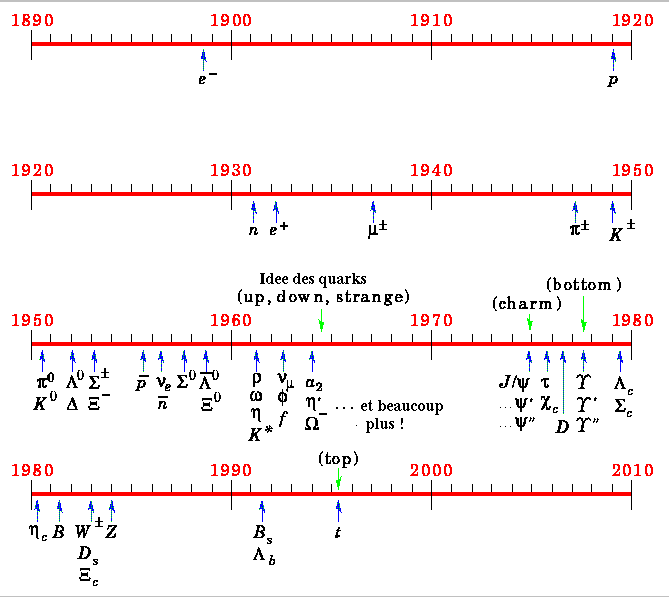
\includegraphics[width=11cm]{Chapter1/Discovery_timeline.png}
\caption{A timeline of particle discoveries.}
\label{fig:Discovery_timeline}
\end{center}
\end{figure}

The astonishing patterns observed in eightfold classification were signalling towards something striking. The explanation arrived in the form of ``Quark Model'',
proposed independently by Gell-Mann~\cite{GellMann:1964nj} and Zweig~\cite{Zweig:570209} in 1964.
They postulated that hadrons are not elementary but composed of fundamental entities, called ``quarks''.
These quarks are present in three flavours: $d$ (down), $u$ (up) and $s$ (strange). Each baryon is made up of three quarks while each meson is made up
of a quark and an anti-quark. Every member of the eightfold supermultiplets
got a quark substructure, however, the states like $\Delta^{++}$ ($uuu$), $\Delta^{-}$ ($ddd$) and $\Omega^{-}$ ($sss$) were appeared to violate the Pauli's exclusion
principle. A way out was proposed by O. W. Greenberg in the
same year by suggesting that each flavour quark further consists of three different color states (red, green and blue), known as color quantum number.
Quarks of different colors combined together in forming the hadrons and all the particles observed in nature are colorless.
This color hypothesis, though did not have any experimental proof, was able to describe the various aspects. 
Indirect searches which includes scattering of electrons with nuclear targets known as ``deep inelastic scattering''~\cite{dokshitzer1977calculation}
(similar to Rutherford's scattering of atom)
were performed in 1967 at SLAC and the first ever evidence of existence of proton substructure was observed.
The Yukawa's meson theory was not applicable for the strong force between quarks, so a new theory of strong force,
known as ``Quantum Chromodynamics'' (QCD) was developed in 1973 by H. Fritzsch and H. Leutwyler, along
with Gell-Mann~\cite{Fritzsch:1973pi}.
They proposed a gauge theory with SU(3) gauge group that predicted the existence of strong force carriers among quarks, termed as ``gluons''. The
first evidence of gluons was obtained at PETRA in 1979 in three-jet events~\cite{Gluons1979}. 

The elementary matter particles known at this stage were: four leptons ($e^{-}$, $\nu_{e}$, $\mu^{-}$, $\nu_{\mu}$) and three quarks ($u$, $d$, $s$).
The existence of a fourth quark, named as ``charm'' ($c$) quark, was predicted by Bjorken and Glashow around 1964~\cite{Bjorken:1964gz},
in order to maintain a symmetry between number of
quarks and leptons. In 1970, more technical aspects were provided for the existence of the charm quark by Glashow, Iliopoulos, and Maiani through GIM
mechanism~\cite{Glashow:1970gm}.
The first evidence of charm quark were obtained in 1974 in the form of $c\bar{c}$ ($J/\psi$) bound state simultaneously by C. C. Ting's
group at BNL~\cite{Aubert:1974js} and
B. Richter's group at SLAC~\cite{Augustin:1974xw}.\ The discovery of $J/\psi$ is known as $\textit{November Revolution}$ in the history.
The Glashow's symmetry that was restored
by the discovery of charm quark was soon broken in 1975 with the observation of a new lepton, known as ``tau'' ($\tau$) lepton,
by M. Perl et.\ al.\ at\ SLAC~\cite{Perl:1975bf}.\
This naturally led scientists to expect for a new family of quarks. Two years later, in 1977, a new heavy meson Upsilon ($\Upsilon$) was discovered by
L. Lederman et.\ al.\ at Fermilab~\cite{Herb:1977ek} and was immediately recognized as the bound state of fifth quark, named as bottom$/$beauty
($b$) quark. After the bottom
quark discovery, the search of its partner, named as truth$/$top ($t$) quark was very much anticipated. However, it took a really long time of 18 years to be finally
discovered in 1995 at Tevatron's CDF~\cite{Abe:1995hr} and D0~\cite{Abachi:1995iq} detectors at fermilab. 

The discovery of the strange particle $K^{+}$ was a startling one. On its first observation in 1947, it appeared to decay in two different
final states, initially thought as two different particles: $\tau^{+}$ (decaying into three $\pi$'s) and $\theta^{+}$ (decaying into two $\pi$'s).
The difference in masses and lifetimes of $\tau$ and $\theta$ were observed to be within experimental errors, but they had different parities~\cite{Lee:1956qn}.
Since parity was considered a universal symmetry then, it led to the famous $\tau$-$\theta$ puzzle
which was solved by the observation of parity violation in weak interactions
by C. S. Wu and collaborators in 1957~\cite{Wu:1957my}. The experimental verification of parity violation led 
to the reformulation of Fermi's theory of $\beta$ decay in terms of
Gamov-Teller transitions. Also, since Fermi's theory was only effective at low energies and found to violate unitarity at high energies, an attempt was
made to devise the theory in terms of intermediate vector particles acting as mediators. The first step was a proposal from C. N. Yang and R. Mills
who in 1954, developed the theory in terms of massless vector particles~\cite{Yang:1954ek}.
But weak interactions required its mediators to be massive, any attempt made to incorporate
masses led to the breaking of local gauge symmetry, thereby making the theory inconsistent. A complete description of weak
interactions was provided by S. Glashow~\cite{Glashow:1961tr}, A. Salam~\cite{Salam:1964ry} and S. Weinberg~\cite{Weinberg:1967tq} 
in terms of electroweak unification, by considering SU(2) $\times$ U(1) gauge group, having three weak gauge bosons denoted by $W^{\pm}$ and $Z$.
They invoked the Higgs mechanism proposed by Higgs~\cite{Higgs:1964ia, Higgs:1964pj, Higgs:1966ev}, Englert $\&$ Brout~\cite{Englert:1964et},
Guralnik, Kibble, $\&$ Hagen~\cite{Guralnik:1964eu} in 1964, that provided masses to gauge bosons by
spontaneous symmetry breaking of local gauge symmetries. The Higgs mechanism also predicted the existence of a new particle named Higgs boson, the mediator of Higgs field. 
The experimental verification of electroweak unification first arrived with the discovery of neutral currents by Gargamelle collaboration in 1973~\cite{Hasert:1973ff}
while performing neutrino scattering experiments, followed by the discovery of weak bosons, $W^{\pm}$~\cite{Arnison:1983rp, Banner:1983jy}
and $Z$~\cite{Arnison:1983mk, Arnison:1983zy, Bagnaia:1983zx} in $p\bar{p}$ collisions at SPS, CERN by UA1 and UA2
collaborations in 1983. The much awaited Higgs boson was finally discovered in 2012 by ATLAS~\cite{Aad:2012tfa} and CMS~\cite{Chatrchyan:2012xdj}
collaborations at CERN, thereby, verifying the source
of mass generation of universal particles. Both the collaborations has extensively studied the properties of this newly
found boson~\cite{CMS:yva, ATLAS:2014yka} and measured the mass to be $m_{H}$ $\approx$ 125 GeV$/$c$^{2}$ within experimental errors.


The SM of particle physics that incorporates six leptons ($e$, $\nu_{e}$, $\mu$, $\nu_{\mu}$, $\tau$, $\nu_{\tau}$),
six quarks ($u$, $d$, $s$, $c$, $b$, $t$) and three fundamental interactions (strong, EM, and weak) alongwith their carriers,
was developed in 1960s \nd\ 1970s. At present, all the particles
hypothesized by SM have been found and are well within the predictions.

\section{Standard Model}
The ``Standard Model'' is the theoretical model of particle physics that encapsulates the fundamental particles and their interactions to provide an ontological basis
to describe the organization of all matter forms except the ones related to gravity. The fundamental particles are classified into two categories:
the matter particles, known as ``fermions'', and the mediators of interactions, known as ``bosons''. In total, SM consists of 17 fundamentals including 12
fermions and 5 bosons. This model, over the years, has been found to be immensely successful in all of its experimental testings.
\subsection{Matter particles}
All the universal matter is made up of fermions, one set of fundamental particles. These fermions carry spin-$\frac{1}{2}$ and can be further
classified into leptons and quarks; each group consisting of six particles related in pairs, thereby forming three generations. 
%The most stable lightest particles form the first generation, with the higher generations formed by the heavier unstable particles.
%All the stable matter of the universe is made up of first generation particles; heavier particles of other generations eventually decay into the next lower generation.

The three quark generation involves: the up ($u$) and down ($d$) quarks, forming 1$^{st}$ generation, followed by the strange ($s$) and charm ($c$) quarks as 2$^{nd}$
generation and the top ($t$) and bottom ($b$) quarks as 3$^{rd}$ generation. These quarks carry fractional charges of $+\frac{2}{3}$e and $-\frac{1}{3}$e, e being the
electronic charge, and exhibit electromagnetic, strong as well as weak forces. Quarks also carry color charge, a property which does not allow them to exist freely
in nature. 

The three generation of leptons are: electron ($e$) and electron neutrino ($\nu_{e}$), muon ($\mu$) and muon neutrino ($\nu_{\mu}$), and tau ($\tau$)
and tau neutrino ($\nu_{\tau}$). Each lepton ($e$, $\mu$, $\tau$) carry one unit of negative charge while corresponding neutrinos are chargeless. SM predicts the
neutrinos to be massless, however, recent discoveries of neutrino oscillations~\cite{Fukuda:1998mi, Fukuda:2001nk, Ahmad:2002jz, Araki:2004mb, Aliu:2004sq, Michael:2006rx} assure that they have small non-zero mass. The leptons take part in electromagnetic and weak interactions while neutrinos involve in weak interactions only.
The three generations of quarks and leptons along with their crucial properties~\cite{Agashe:2014kda} are summarized in \tab{\ref{Table:SMparticles}}.
\begin{table}[h!]
\begin{center}
\resizebox{15cm}{!}{
%\begin{tabular}{c !{\vrule width -1pt}c !{\vrule width -1pt}c !{\vrule width -1pt}c !{\vrule width -1pt}c !{\vrule width -1pt}c !{\vrule width -1pt}c !{\vrule width -1pt}c}
\begin{tabular}{cccccccc}
\toprule
\belowrulesepcolor{Mygray}
\belowrulesepcolor{Mygray}
\belowrulesepcolor{Mygray}
\rowcolor{Mygray}[\dimexpr\tabcolsep+0.09pt\relax]
& \multicolumn{3}{c}{Leptons} & \phantom{abc} & \multicolumn{3}{c}{Quarks} \\
\aboverulesepcolor{Mygray}
\aboverulesepcolor{Mygray}
\aboverulesepcolor{Mygray}
%\arrayrulecolor{Mygray} \specialrule{0.1pt}{0pt}{-0.01pt} \arrayrulecolor{black} 
%\arrayrulecolor{Mygray}
%\cmidrule[0.1pt](r){1-1} \cmidrule[0.01pt](lr){5-5}
\rowcolor{Mygray}[\dimexpr\tabcolsep+0.09pt\relax]
& Flavor & Charge & Mass (MeV$/$C$^{2}$) && Flavor & Charge & Mass (MeV$/$C$^{2}$) \\
\aboverulesepcolor{Mygray}
\aboverulesepcolor{Mygray}
\aboverulesepcolor{Mygray}
\midrule
$1^{st}$ Generation \\
 & $e$ & -1 & 0.511 && $u$ & $+$\sfrac{2}{3} & $\sim2.2$ \\
 & $\nu_{e}$    &  0 & $<2.2\times10^{-6}$ && $d$ & $-$\sfrac{1}{3} & $\sim4.7$  \\
$2^{nd}$ Generation \\
 & $\mu$        & -1 & 105.7 && $c$ & $+$\sfrac{2}{3} & $\sim1.27\times10^{3}$  \\
 & $\nu_{\mu}$  &  0 & $<0.17$ && $s$ & $-$\sfrac{1}{3} & $\sim96$  \\
$3^{rd}$ Generation \\
 & $\tau$       & -1 & 1776.9 && $t$ & $+$\sfrac{2}{3} & $\sim173.21\times10^{3}$  \\
 & $\nu_{\tau}$ &  0 & $<18.2$ && $b$ & $-$\sfrac{1}{3} & $\sim4.18\times10^{3}$  \\
\bottomrule
\end{tabular}
}
\caption{Standard model fundamental fermion's three generations.}
\label{Table:SMparticles}
\end{center}
\end{table}
\vspace{-0.3in}

%%%%%%%%%%%%%%%%%%%%%%%%%%%%%%%%%%%%%%%%%%%%%%%%%%%%%%%%%%%%%%%%%%%%%%%%%%%%%%%%%%%%%%%%%%%%%%%%%%%%%%%%%%%%%%%%%%%%%%%%%%%%%%%%%%%%%%%%%%%%%%%%%%%
%% %---------------TABLE FOR MC samples-------------------                                                                                       %%
%% \definecolor{Gray}{gray}{0.9}                                                                                                                 %%
%% \begin{table}[h!]                                                                                                                             %%
%% \begin{center}                                                                                                                                %%
%% %\begin{ruledtabular}                                                                                                                         %%
%% \resizebox{16cm}{!}{                                                                                                                          %%
%% \begin{tabular}{@{}ccccccc@{}}                                                                                                                %%
%%   \hline                                                                                                                                      %%
%%   \rowcolor{Gray}                                                                                                                             %%
%%   &\multicolumn{3}{c||}{Leptons$\left(\text{spin}=\frac{1}{2}\right)$} & \multicolumn{3}{c|}{Quarks$\left(\text{spin}=\frac{1}{2}\right)$} \\ %%
%%   \cline{2-7}                                                                                                                                 %%
%% Generation & Flavor & Charge & Mass (MeV/c$^{2}$) &  Flavor & Charge & Mass (MeV/c$^{2}$) \\                                                  %%
%% \hline                                                                                                                                        %%
%%    & $e$          & -1 & 0.511               & $u$ & +2/3 & $\sim2.3$  \\                                                                     %%
%% 1  & $\nu_{e}$    &  0 & $<2.2\times10^{-6}$ & $d$ & -1/3 & $\sim4.8$  \\                                                                     %%
%% \hline                                                                                                                                        %%
%%    & $\mu$        & -1 & 105.7               & $c$ & +2/3 & $\sim1.27\times10^{3}$  \\                                                        %%
%% 2  & $\nu_{\mu}$  &  0 & $<0.17$             & $s$ & -1/3 & $\sim95$  \\                                                                      %%
%% \hline                                                                                                                                        %%
%%    & $\tau$       & -1 & 1777                & $t$ & +2/3 & $\sim173.21\times10^{3}$  \\                                                      %%
%% 3  & $\nu_{\tau}$ &  0 & $<15.5$             & $b$ & -1/3 & $\sim4.18\times10^{3}$  \\                                                        %%
%% \hline                                                                                                                                        %%
%% \end{tabular}                                                                                                                                 %%
%% }                                                                                                                                             %%
%% \caption{Three generation of elementary particles in the SM~\cite{Agashe:2014kda}.}                                                           %%
%% %\end{ruledtabular}                                                                                                                           %%
%%    \label{Table:SMparticles}                                                                                                                  %%
%% \end{center}                                                                                                                                  %%
%% \end{table}                                                                                                                                   %%
%%%%%%%%%%%%%%%%%%%%%%%%%%%%%%%%%%%%%%%%%%%%%%%%%%%%%%%%%%%%%%%%%%%%%%%%%%%%%%%%%%%%%%%%%%%%%%%%%%%%%%%%%%%%%%%%%%%%%%%%%%%%%%%%%%%%%%%%%%%%%%%%%%%

For each particle listed in table above, corresponding anti-particle having same mass and spin but opposite charge exists. 
\subsection{Forces and messenger particles}
All universal phenomena exhibit and experience four different kind of forces: strong, weak, electromagnetic and gravitational.
The gravity and electromagnetic interaction are the only two forces that can be experienced in day-to-day life.  
Strong and weak forces are applicable at sub-nuclear level only.
Standard model describes each force, except gravity, in the form of a physical theory, known as the Quantum Field Theory (QFT).
These theories are based on the analogy of exchange forces via mediators, the spin-1 bosons; another set of fundamental particles.
These mediators for electromagnetic interaction are ``photons'' whereas for strong force are ``gluons'' and for weak force are
``intermediate vector bosons'' $W^{\pm}$ and $Z$.  These forces operate between particles due to different charges: EM $\rightarrow$
electric charge, Strong $\rightarrow$ color charge, Weak $\rightarrow$ flavor charge. The \tab{\ref{Table:SMforces}} summarize the important
properties~\cite{Agashe:2014kda} of all the forces.

\begin{table}[h!]
\begin{center}
\resizebox{15cm}{!}{
%\begin{tabular}{c !{\vrule width -1pt}c !{\vrule width -1pt}c !{\vrule width -1pt}c !{\vrule width -1pt}c !{\vrule width -1pt}c !{\vrule width -1pt}c !{\vrule width -1pt}c}  %%% !{\vrule width -1pt} to make column line width less, so that white space not visible in colored table. but not working very nicely.
\begin{tabular}{cccccccc}
\toprule
\belowrulesepcolor{Mygray}
\belowrulesepcolor{Mygray}
\belowrulesepcolor{Mygray}
\rowcolor{Mygray}[\dimexpr\tabcolsep+0.09pt\relax]  
Force  & Mediator & Charge & Mass  & Range  & Rel.  & Long distance \\
\aboverulesepcolor{Mygray}
\aboverulesepcolor{Mygray}
\rowcolor{Mygray}[\dimexpr\tabcolsep+0.09pt\relax]
&          &        & (GeV$/$C$^{2}$) & (m) & Strength & behavior \\
\aboverulesepcolor{Mygray}
\aboverulesepcolor{Mygray}
\aboverulesepcolor{Mygray}
\midrule
Strong & Gluons ($g$) & 0 & 0   & $10^{-15}$ & 1 & $\sim$ r   \\
Electromagnetic & Photon ($\gamma$) & 0 & 0  & $\infty$ & $\sfrac{1}{137}$ & $\sfrac{1}{r^{2}}$ \\
Weak            & $W^{\pm}$  & $\pm1$ & 80.38 & $10^{-18}$ & $10^{-5}$  & $\sfrac{1}{r}e^{-mr}$  \\
                & $Z^{0}$    & 0      & 91.18 & & &  \\   
Gravity         & Graviton ($G$) & 0  & 0  & $\infty$ & $10^{-38}$ & $\sfrac{1}{r^{2}}$   \\
\bottomrule
\end{tabular}
}
\caption{Important properties of fundamental forces of universe.}
\label{Table:SMforces}
\end{center}
\end{table}
\vspace{-0.3in}


The electromagnetic interaction is the unification of electric and magnetic forces, first formulated in 1864 by Maxwell. The QFT of electromagnetic forces is known
as Quantum Electrodynamics (QED)~\cite{Feynman:1948ur, Feynman:1948km, Tomonaga:1948zz, Schwinger:1948iu, Schwinger:1948yk, Dyson:1949bp, Peskin:1995ev},
perfected by Feynman, Tomonaga, and Schwinger in the 1940s. EM interactions are of infinite range, thereby requiring its mediator (photon) to be massless.
The magnitude of this interaction is defined by means of a coupling constant,
$\alpha(Q^{2})= \frac{\alpha(\mu^{2})}{ 1 - \frac{\alpha(\mu^{2})}{3\pi}\text{log}\left(\frac{Q^{2}}{\mu^{2}}\right)}$
where $\mu$ is the typical scale of renormalization. The interaction strength increases with the increase of interaction energy and decrease of interaction length.

%\begin{equation}
%\alpha(Q^{2})= \frac{\alpha(\mu^{2})}{ 1 - \frac{\alpha(\mu^{2})}{3\pi}\text{log}\left(\frac{Q^{2}}{\mu^{2}}\right)},
%\label{eg:QEDalpha}
%\end{equation}

The weak force is answerable for existence of life on earth owing to its radioactive decays. It is actually the only force responsible for decay of particles.
It is also called Quantum Flavourdynamics (QFD) because of its capability of changing the flavour of quarks.
The first ever theory of weak forces was represented by Fermi in 1934;
later refined by Feynman and Gell-mann and finally, presented in its current scheme by Glashow, Weinberg, and Salam,
in 1960s~\cite{Glashow:1961tr, Salam:1964ry, Weinberg:1967tq}, in the form of Electroweak theory. This theory envision the unification of electromagnetic
and weak forces at some higher energy regime, thereby, predicting the existence of massive weak bosons, $W^{\pm}$ and $Z$.
The mechanism that is responsible for providing mass to weak bosons is known as Higgs mechanism that also predict the existence of one more fundamental boson called
Higgs boson. The magnitude of weak forces is found to depend on the coupling strength of weak bosons as well as their masses. 

The strong force is the mechanism responsible for the binding of quarks inside protons and neutrons, thereby, ensuring the stability of nucleus.
Most of the mass of a proton (or neutron) arises from the field energy provided by the strong force, the contribution of quark mass is almost negligible
in total proton's mass.
The field theory of strong force is known as Quantum Chromodynamics (QCD) that explains the interaction mechanism of strong force in the form of exchange of massless
gluons. The gluons interact with quarks as well as other gluons by means of a charge known as color charge. Color charge is analogous to electric charge 
but it comes in three different types. 
The behaviour of partons\footnote{Together quarks and gluons are referred to as partons} within the nucleons are determined by the properties of asymptotic
freedom and confinement. The coupling constant~\cite{Kluth:2006vf} determining the QCD interaction strength is given by,
\begin{equation}
\alpha_{s}(Q^{2})= \frac{12\pi}{(11\textrm{c}-2\textrm{n}_{\textrm{f}})\ln\left(\frac{Q^{2}}{\Lambda^{2}}\right)}
\label{eg:alpha_s}
\end{equation}
where $Q$ is the momentum transferred, c is the total number of quark colors (\ie 3), n$_{\textrm{f}}$ is the total number of quark flavors (\ie 6),
$\Lambda$ is the chromodynamics scale, which is given by:
\begin{equation}
\Lambda^{2}  = \mu^{2} \left[  \frac{-12\pi}{(11\textrm{c}-2\textrm{n}_{\textrm{f}}) \alpha_{s}(\mu^{2})  } \right]
\end{equation}
where $\mu$ is the renormalization scale. For $Q^{2}\to\infty$ and hence distance $\to0$, $\alpha_{s}(Q^{2})\to0$, which means that at high
energies with large momentum transfers in the interactions ($Q^{2}\gg\Lambda^{2}$), the coupling strength between the partons decreases, thereby making
the quarks and gluons to behave as free particles inside the nucleus. This property of quarks is referred to as
``asymptotic freedom''~\cite{Gross:1973ju,Gross:1974cs,Politzer:1974fr}.
For low $Q^{2}$, partons form hadronic bound states and can not be observed in isolated form. This attribute is referred to as ``quark confinement''. 


\subsection{SM as a gauge theory}
The standard model has been established on the notion of ``symmetry''. As per the statement of the Noether's theorm: the continuous symmetries of a system are
associated with conservation laws. For example, invariance of the laws of physics under space and time transformations, refer to as the symmetries of nature,
leads to the conservation of momentum and energy. These symmetry transformations of a system can be easily modelled in the form of
mathematical group representations, like the rotational symmetry of a system in n-dimension form the group representation for the special orthogonal group $SO (n)$.

A symmetry can be labelled as a global or local symmetry depending upon whether the transformation is same or different for each space-time point.
A physical theory of a system constructed by requiring local symmetries is known as ``gauge theory'', while the corresponding symmetry transformations
are called ``gauge transformations''.
The corresponding associated group representation is known as ``gauge group''. The gauge theory is called non-abelian if
the underlying gauge group is non-commutative. In SM, a physical system is described in terms of a Lagrangian which is then required to remain invariant
under a local gauge transformation. This requirement leads to the appearance of additional fields (known as ``gauge fields'') in the Lagrangian that
couples with the particles of the system, thereby generating the fundamental interactions. The number of gauge fields
in a gauge theory is determined by the dimension of the gauge group and the quanta of these gauge fields are known as the ``gauge bosons''.

The standard model portray the three fundamental forces in the form of gauge theories and unifies them as a non-abelian gauge theory under
$SU (3)_{color}$ $\otimes$ $SU (2)_{flavor}$ $\otimes$ $U (1)_{charge}$ gauge group. A more detailed description of this formalism is outlined as:

\subsubsection{Quantum electrodynamics}
Quantum electrodynamics is the abelian gauge theory of electromagnetic interactions characterized by the symmetry group $U (1)$.
The dynamics of a free particle of spin-$\frac{1}{2}$ can be represented in terms of Dirac Lagrangian,
\begin{equation}
\mathcal{L}_{\Psi} = \overline{\Psi}(x)(i\gamma^{\mu}\partial_{\mu} - m){\Psi}(x)
\label{eq:QEDLang}
\end{equation}
where $\Psi(x)$ is the Dirac field and $\gamma^{\mu}$ are the $4\times4$ Dirac matrices. We define a symmetry operation of the global phase transformations:
\begin{equation}
\Psi(x) \rightarrow \Psi^{\prime}(x) = e^{i{\alpha}}\Psi(x) \hspace{0.2 in}; \hspace{0.4 in} \overline{\Psi}(x) \rightarrow \overline{\Psi^{\prime}}(x) = e^{-i{\alpha}}\overline{\Psi}(x)
\label{eg:Globalphase}
\end{equation}
where phase $\alpha$ is independent of the spacetime variation. The Lagrangian remains invariant under this transformation, $\Delta\mathcal{L}$ = 0.
As per the statement of Noether's theorm, this invariance corresponds to a current $j^{\mu}$, known as Noether's current, defined by,
\begin{equation}
j^{\mu} = \frac{\partial\mathcal{L}}{\partial(\partial_{\mu}\Psi)}\delta\Psi \propto \overline{\Psi}\gamma^{\mu}{\Psi},
\label{eg:jmu}
\end{equation}
which remains conserved, that is, $\partial_{\mu}j^{\mu}$ = $0$. Now, if the phase is made to vary locally as a function of spacetime points, such that
\begin{equation}
\Psi(x) \rightarrow \Psi^{\prime}(x) = e^{i{\alpha}(x)}\Psi(x) \hspace{0.2 in}; \hspace{0.4 in} \overline{\Psi}(x) \rightarrow \overline{\Psi^{\prime}}(x) = e^{-i{\alpha}(x)}\overline{\Psi}(x)
\label{eg:Localphase}
\end{equation}
then under this symmetry operation, the Lagrangian transforms as:
\begin{equation}
\mathcal{L}_{\Psi} \rightarrow \mathcal{L}'_{\Psi} = \mathcal{L}_{\Psi} - \overline{\Psi}{\gamma}^{\mu}{\Psi}{\partial}_{\mu}{\alpha}(x) 
\label{eg:LangInLocalPhase}
\end{equation}
which is no longer invariant. In in attempt to achieve invariance, we introduce a covariant derivative $D_{\mu}$ and a new gauge field $A_{\mu}$ such as
\begin{equation}
\partial_{\mu} \rightarrow D_{\mu} = \partial_{\mu} - ieA_{\mu} \hspace{0.2 in} ; \hspace{0.4 in} A_{\mu} \rightarrow A^{\prime}_{\mu} = A_{\mu} + \frac{1}{e}\partial_{\mu}\alpha(x)
\label{eg:delToD}
\end{equation}
%\begin{equation}
%\label{eg:Amu}
%x\end{equation}
Under this transformation, the Lagrangian changed as
\begin{equation}
\begin{split}
  \mathcal{L}_{\Psi} \rightarrow \mathcal{L}^{\prime}_{\Psi} & = \overline{\Psi^{\prime}}(i\gamma^{\mu}D_{\mu} - m){\Psi^{\prime}} \\
  & = \overline{\Psi}e^{-i\alpha(x)}(i\gamma^{\mu}(\partial_{\mu} - ieA^{\prime}_{\mu}) - m)e^{i\alpha(x)}{\Psi} \\
  & = \overline{\Psi}e^{-i\alpha(x)}(i\gamma^{\mu}\partial_{\mu} + e\gamma^{\mu}(A_{\mu} + \frac{1}{e}\partial_{\mu}\alpha(x)) - m)e^{i\alpha(x)}{\Psi} \\
  & = \overline{\Psi}(i\gamma^{\mu}\partial_{\mu} - m){\Psi} + e\overline{\Psi}\gamma^{\mu}A_{\mu}{\Psi} \\
  & = \mathcal{L}_{\Psi} + e\overline{\Psi}\gamma^{\mu}A_{\mu}{\Psi}
  \label{eg:newLang}
\end{split}
\end{equation}
which is invariant under the local gauge transformation defined in \eqn{\ref{eg:Localphase}}.

Demanding local gauge invariance under the gauge group $U (1)$ has resulted into the introduction of gauge field $A_{\mu}$ which is none other than the required
electromagnetic field, also called the photon field, and it couples with Dirac particles ($e^{-}$s) through the term $e\overline{\Psi}\gamma^{\mu}A_{\mu}{\Psi}$. Since $A_{\mu}$ is a physical field, we
must introduce a gauge invariant kinetic energy term for this, given by 
\begin{equation}
  \mathcal{L}_{K.E.} = -\frac{1}{4}F^{\mu\nu}F_{\mu\nu}
  \label{eg:Lke}
\end{equation}
where $F_{\mu\nu}$ = $\partial_{\mu}A_{\nu} - \partial_{\nu}A_{\mu}$, known as the electromagnetic strength tensor. Adding this term, the complete gauge invariant
Lagrangian for electromagnetic interactions can be written as:
\begin{equation}
  \begin{split}
  & \mathcal{L}_{total} = \mathcal{L}_{free} + \mathcal{L}_{int} + \mathcal{L}_{K.E} \\
  & \mathcal{L}_{total} = \overline{\Psi}(i\gamma^{\mu}\partial_{\mu} - m){\Psi} + e\overline{\Psi}\gamma^{\mu}A_{\mu}{\Psi} - \frac{1}{4}F^{\mu\nu}F_{\mu\nu}
    \label{eg:Lcomp}
    \end{split}
\end{equation}

If a mass term, like $m^{2}A_{\mu}A^{\mu}$, is considered for field $A_{\mu}$, it will again spoil the gauge invariance. So this term is prohibited in the QED
Lagrangian and corresponding gauge particle, the photon, remain massless. The interaction term in the Lagrangian, $e\overline{\Psi}\gamma^{\mu}A_{\mu}{\Psi}$ can
also be written as $-j^{\mu}A_{\mu}$ where $j^{\mu}$ = $-e\overline{\Psi}\gamma^{\mu}{\Psi}$, known as the current density, $-e$ being the electric charge.
The current density $j^{\mu}$ is a conserved quantity of electromagnetic interactions.

\subsubsection{Electroweak}
The electroweak theory is a unified theory of electromagnetic and weak interactions. This theory came into existence in an attempt to derive a self-consistent
invariant gauge theory for weak interactions, analogous to QED.\ The weak interactions were first proposed by Fermi in 1934 as an explanation
of $\beta$-decay. He came up with the following interaction Lagrangian for $\beta$-decay process:
\begin{equation}
\mathcal{L}_{w} = G_{F}(\overline{\Psi}_{p}\gamma_{\mu}{\Psi}_{n})(\overline{\Psi}_{e}\gamma^{\mu}{\Psi}_{\nu})
\end{equation}
where $G_{F}$ is the Fermi coupling constant and ${\Psi}_{p}$, ${\Psi}_{n}$, ${\Psi}_{e}$, ${\Psi}_{\nu}$ are the particle fields.
In his proposal, Fermi considered the interaction of four fermions at one point, known as contact interaction. The most remarkable difference in Fermi Lagrangian
was the presence of charged currents, contrary to neutral current of QED.\

The observation of parity violation in weak interactions emphasized that weak interactions involve only left-handed fermions and right-handed anti-fermions
(observed experimentally in 1958 by Goldhaber et.\ al.~\cite{Goldhaber:1958nb}) and led to the introduction of axial-vector terms in the Fermi Lagrangian,
\begin{equation}
\mathcal{L}_{w} = \frac{G_{F}}{\sqrt{2}}(\overline{\Psi}_{p}\gamma_{\mu}(1 - g_{A}\gamma_{5}){\Psi}_{n})(\overline{\Psi}_{e}\gamma^{\mu}(1 - \gamma_{5}){\Psi}_{\nu})
\end{equation}
where $g_{A}$ = $|\frac{G_{A}}{G_{V}}|$, $G_{V}$ and $G_{A}$ being the constants for vector and axial-vector couplings respectively.
%In the formation of this Lagrangian, the projection operators, $P_{L}$ = $\frac{1 - \gamma^{5}}{2}$ and $P_{R}$ = $\frac{1 + \gamma^{5}}{2}$ were introduced
%having the properties: $P^{2}_{L} = P_{L}$, $P^{2}_{R} = P_{R}$, $P_{L}P_{R} = 0$ and $\gamma^{\mu}P_{L} = P_{R}\gamma^{\mu}$.
%Their operation on the fermionic fields, $P_{L}\Psi$ = $\Psi_{L}$ ($\overline{\Psi}P_{L}$ = $\overline{\Psi}_{R}$) and
%$P_{R}\Psi$ = $\Psi_{R}$ ($\overline{\Psi}P_{R}$ = $\overline{\Psi}_{L}$), results into left and right projections. The importance of these projection operators can be
%considered from the fact that
%\begin{equation}                                                                                                                           
%\begin{split}                                                                                                                              
%  \overline{\Psi}_{e}\gamma^{\mu}\left(\frac{1 - \gamma_{5}}{2}\right){\Psi}_{\nu} & = \overline{\Psi}_{e}\gamma^{\mu}P_{L}{\Psi}_{\nu}  
%  = \overline{\Psi}_{e}\gamma^{\mu}P^{2}_{L}{\Psi}_{\nu}  %(using the property, P^{2}_{L} = P_{L})\\                                    
%  = \overline{\Psi}_{e}P_{R}\gamma^{\mu}P_{L}{\Psi}_{\nu}  %(using, \gamma^{\mu}\gamma^{5} = -\gamma^{5}\gamma^{\mu})\\                 
%  = \overline{\Psi}_{eL}\gamma^{\mu}{\Psi}_{{\nu}L} %(using, \overline{\Psi}P_{R} = \overline{\Psi_{L}})\\                              
%\label{eg:projection}                                                                                                                      
%\end{split}                                                                                                                                
%\end{equation}                                                                                                                             
%implying that only left-handed fermions experience weak interactions.
However, this $V - A$ theory was still incomplete in the sense that
it could not be renormalized and violated unitarity at high energies.

Later on, in 1960s, it was observed independently by Glashow, Salam and Weinberg~\cite{Glashow:1961tr, Salam:1964ry, Weinberg:1967tq}
that a gauge-invariant theory for the weak interactions can be constructed if electromagnetic interactions are also included under the gauge group
${SU(2)}_{L} \times {U(1)}_{Y}$. The group ${SU(2)}_{L}$, where $L$ refers to left-handed,
forms the gauge group of weak interactions and considers the doublet of left-handed lepton (or an up-type quark)
and lepton neutrino (or a down-type quark) as its fundamental representation under the weak isospin, $T$ = $\frac{1}{2}$,
which remains conserved under this group transformation.
The group ${U(1)}_{Y}$ form the gauge group under the weak hypercharge, $Y$.  
The weak isospin's $3^{rd}$ component, $T_{3}$
and weak hypercharge, $Y$ are related to the electric charge, $Q$ by the Gell-Mann-Nishijima relation~\cite{Nakano:1953zz, Nishijima:1955zz, Gell-Mann:1956iqa}:
$Q = T_{3} + \frac{Y}{2}$. The \tab{\ref{tab:EWK_fermions}} summarize the electroweak singlets and doublets and the various quantum numbers associated with them.

%\begingroup\setlength{\fboxsep}{0pt}
%\colorbox{lightgray}{%
\begin{table}[h]
\begin{center}
\resizebox{11.5cm}{!}{    
\begin{tabular}{ccccccc}
\toprule
\belowrulesepcolor{Mygray}
\belowrulesepcolor{Mygray}
\belowrulesepcolor{Mygray}
\rowcolor{Mygray}[\dimexpr\tabcolsep+0.09pt\relax]
 \multicolumn{3}{c}{Fermions: Singlets \& Doublets} & $Q$ & $T$ & $T_{3}$ & $Y$ \\
\aboverulesepcolor{Mygray}
\aboverulesepcolor{Mygray}
\aboverulesepcolor{Mygray}
\midrule
%\rowcolor{black!20}
$                    
\left(               
\begin{array}{c}     
{\nu}_{e}\\          
e^{-}\\              
\end{array}          
\right)_{L}          
$ &                  
$                    
\left(               
\begin{array}{c}     
{\nu}_{\mu}\\        
{\mu}^{-}\\          
\end{array}          
\right)_{L}          
$ &                  
$                    
\left(               
\begin{array}{c}     
{\nu}_{\tau}\\       
{\tau}^{-}\\         
\end{array}          
\right)_{L}          
$ &                  
$                    
\begin{array}{c}     
0\\                  
-1\\                 
\end{array}          
$ &                  
$                    
\begin{array}{c}     
\sfrac{1}{2}\\                
\sfrac{1}{2}\\                
\end{array}          
$ &                  
$                    
\begin{array}{c}     
\sfrac{1}{2}\\                
-\sfrac{1}{2}\\               
\end{array}          
$ &                  
$                    
\begin{array}{c}     
-1\\                 
-1\\                 
\end{array}          
$ \\                 
\\                   
$                    
\left(               
\begin{array}{c}     
u\\                  
d\\                  
\end{array}          
\right)_{L}          
$ &                  
$                    
\left(               
\begin{array}{c}     
c\\                  
s\\                  
\end{array}          
\right)_{L}          
$ &                  
$                    
\left(               
\begin{array}{c}     
t\\                  
b\\                  
\end{array}          
\right)_{L}          
$ &                  
$                    
\begin{array}{c}     
\sfrac{2}{3}\\                
-\sfrac{1}{3}\\               
\end{array}          
$ &                  
$                    
\begin{array}{c}     
\sfrac{1}{2}\\                
\sfrac{1}{2}\\                
\end{array}          
$ &                  
$                    
\begin{array}{c}     
\sfrac{1}{2}\\                
-\sfrac{1}{2}\\               
\end{array}          
$ &                  
$                    
\begin{array}{c}     
\sfrac{1}{3}\\                
\sfrac{1}{3}\\                
\end{array}          
$ \\                 
\\
$e_{R}$ & $\mu_{R}$ & $\tau_{R}$ & $-1$ & $0$ & $0$ & $-2$ \\
$u_{R}$ & $c_{R}$ & $t_{R}$ & $\sfrac{2}{3}$ & $0$ & $0$ & $\sfrac{4}{3}$ \\
$d_{R}$ & $s_{R}$ & $b_{R}$ & $-\sfrac{1}{3}$ & $0$ & $0$ & $-\sfrac{2}{3}$ \\
\bottomrule
\end{tabular}
}
\caption{Assignment of the various quantum numbers including $T_{3}$ and $Y$ to the electroweak singlet and doublet fundamental fermions.}
\label{tab:EWK_fermions}
\end{center}
\end{table}


\vspace{-0.2in}
If we consider only the first generation quarks and leptons, then
\begin{equation}
\Psi_{L} = 
\left(
\begin{array}{c}
\nu_{e^{-}}\\
e^{-}\\
\end{array}
\right)_{L}
\hspace{0.2cm} or \hspace{0.2cm}\left(
\begin{array}{c}
u \\
d \\
\end{array}
\right)_{L}
\hspace{0.3cm}; \hspace{0.4cm} \Psi_{R} = e^{-}_{R}, \hspace{0.1cm} u_{R}, \hspace{0.1cm} d_{R}
\end{equation}
form the left-handed and right-handed particle fields. The free particle Lagrangian for these fields can be written as,
\begin{equation}
\mathcal{L}_{free} = \overline{\Psi}_{L}(i\gamma^{\mu}\partial_{\mu} - m){\Psi}_{L} + \overline{\Psi}_{R}(i\gamma^{\mu}\partial_{\mu} - m){\Psi}_{R}
\label{eg:EWfree}
\end{equation}
which remains invariant under the following global gauge transformations:
\begin{equation}
  \begin{split}
   \Psi_{L} \rightarrow \Psi^{\prime}_{L} = e^{i{\alpha_{a}}T^{a}+i{\beta}\frac{Y}{2}}{\Psi_{L}} \hspace{0.2 in} ; \hspace{0.4 in} 
  %\overline{\Psi}_{L} \rightarrow \overline{\Psi^{\prime}}_{L} = e^{-i{\alpha_{a}}T^{a}-i{\beta}Y}\overline{\Psi}_{L} \\
   \Psi_{R} \rightarrow \Psi^{\prime}_{R} = e^{i{\beta}\frac{Y}{2}}{\Psi_{R}} %\hspace{0.56in} ; \hspace{0.4 in} 
  %\overline{\Psi}_{R} \rightarrow \overline{\Psi^{\prime}}_{R} = e^{-i{\beta}Y}\overline{\Psi}_{R}
  \label{eg:EWKGlobalphase}
  \end{split}
\end{equation}
where $T_a$ and $Y$ are the generators of $SU(2)$ and $U(1)$ transformations with $T_a$ = $\sigma_{a}/2$,
$\sigma_{a}$ are the Pauli spin matrices\footnote{Pauli matrices are a set of three 
$2\times2$ hermitian and unitary complex matrices, given as:
\newline
$\sigma_{1} = \left(\begin{array}{cc} 0 & 1 \\ 1 & 0 \end{array}\right),\:\:\:
\sigma_{2} = \left(\begin{array}{cc} 0 & -i \\ i & 0 \end{array}\right),\:\:\:
\sigma_{3} = \left(\begin{array}{cc} 1 & 0 \\ 0 & -1 \end{array}\right).$}
for $a$ = 1,2,3. However, the invariance
of Lagrangian is carried away when the phases $\alpha$ and $\beta$ are made to vary as a function of spacetime points. In order to restore the invariance,
the following covariant derivatives and fields are introduced:
\begin{equation}
  \begin{split}
    & \partial_{\mu} \rightarrow D_{\mu} = \partial_{\mu} - igT_{a}W_{\mu}^{a} - ig^{\prime}\frac{Y}{2}B_{\mu} & & \textrm{for SU(2) doublets}\\
    & \partial_{\mu} \rightarrow D_{\mu} = \partial_{\mu} - ig^{\prime}\frac{Y}{2}B_{\mu} & & \textrm{for U(1) singlets}
    \label{eg:EWKdelToD}
    \end{split}
\end{equation}
where the fields $W_{\mu}$ and $B_{\mu}$ varies as
\begin{equation}
W_{\mu} \rightarrow W^{\prime}_{\mu} = W_{\mu} + \frac{1}{g}\partial_{\mu}\alpha(x) - \alpha(x) \times W_{\mu} \hspace{0.2in} ; \hspace{0.4in} B_{\mu} \rightarrow B^{\prime}_{\mu} = B_{\mu} + \frac{1}{g^{\prime}}\partial_{\mu}\beta(x) 
\label{eg:EWKfields}
\end{equation}
Under these covariant transformations, the Lagrangian achieve invariance as:
\begin{equation}
\begin{split}
  \mathcal{L}_{free} \rightarrow \mathcal{L}^{\prime}_{free} = \mathcal{L}_{fermion} & = \mathcal{L}_{free} + g\overline{\Psi}_{L}\gamma^{\mu}T_{a}W_{\mu}^{a}{\Psi_{L}} + g^{\prime}\frac{Y}{2}B_{\mu}(\overline{\Psi}_{L}\gamma^{\mu}{\Psi_{L}} + \overline{\Psi}_{R}\gamma^{\mu}{\Psi_{R}}) \\
  & = \mathcal{L}_{free} + g\overline{\Psi}_{L}\gamma^{\mu}T_{a}W_{\mu}^{a}{\Psi_{L}} + g^{\prime}\overline{\Psi}\gamma^{\mu}\frac{Y}{2}B_{\mu}{\Psi} \\
  & = \overline{\Psi}_{L}(i\gamma^{\mu}D_{\mu} - m){\Psi}_{L} + \overline{\Psi}_{R}(i\gamma^{\mu}D_{\mu} - m){\Psi}_{R}
  \label{eg:newLang}
\end{split}
\end{equation}
where $T_{a}W_{\mu}^{a}$ = $\frac{\sigma_{a}}{2}.W_{\mu}^{a}$ = $\frac{1}{2}(\sigma_{1}W_{\mu}^{1} + \sigma_{2}W_{\mu}^{2} + \sigma_{3}W_{\mu}^{3})$. Replacing the 
Pauli matrices with the matrix form, and using $W_{\mu}^{\pm}$ = $(W_{\mu}^{1} \mp iW_{\mu}^{2})/{\sqrt{2}}$,  
\begin{equation}
  \begin{split}
     T_{a}W_{\mu}^{a} = \frac{1}{2}\left(\begin{array}{lr} W_{\mu}^{3}  &W_{\mu}^{1} - iW_{\mu}^{2} \\ W_{\mu}^{1} + iW_{\mu}^{2}  & -W_{\mu}^{3} \end{array} \right) =
    \frac{1}{2}\left(\begin{array}{lr} W_{\mu}^{3}  &\sqrt{2}W_{\mu}^{+} \\ \sqrt{2}W_{\mu}^{-} & -W_{\mu}^{3} \end{array} \right)
\label{eg:Wmus}
\end{split} 
\end{equation}

Thus, the invariance under local gauge transformations led to the introduction of four gauge bosons into the theory: a positively charged $W^{{\mu}+}$,
a negatively charged $W^{{\mu}-}$ and two neutrals $W^{{\mu}3}$, and $B^{\mu}$ where $W_{\mu}$'s interacts with only the left-handed fermions while $B_{\mu}$
interacts with both left and right handed. The kinetic energy terms for the gauge fields can be written as,
\begin{equation}
  \begin{split}
    & \mathcal{L}_{K.E.} = -\frac{1}{4}W^{{\mu\nu}a}W_{\mu\nu}^{a} -\frac{1}{4}B^{\mu\nu}B_{\mu\nu} & & \textrm{where,} \\
    & W^{a}_{\mu\nu} = \partial_{\mu}W_{\nu}^{a} - \partial_{\nu}W_{\mu}^{a} -g\epsilon_{abc}W_{\mu}^{b}W_{\nu}^{c}, & & \epsilon_{abc} \textrm{ is totally anti-symmetric tensor}\\
    & B_{\mu\nu} = \partial_{\mu}B_{\nu} - \partial_{\nu}B_{\mu}
    \label{eg:EWK_Lke}
    \end{split}
\end{equation}
The corresponding weak current densities that will remain conserved under $SU(2)$ $\times$ $U(1)$ are represented as:
\begin{equation}
  \begin{split}
    & j_{\mu}^{T} = -g\overline{\Psi}_{L}\gamma_{\mu}T{\Psi}_{L} \hspace{0.2in} ; \hspace{0.4in} j_{\mu}^{Y} = -g^{\prime}\overline{\Psi}\gamma_{\mu}Y{\Psi}
    \label{eg:EWK_jmu}
  \end{split}
\end{equation}
Using the general form of electromagnetic current, $j_{\mu}^{em} = -e\overline{\Psi}\gamma_{\mu}Q{\Psi}$, where $Q$ is the charge operator for EM
interactions, and Gell-Mann-Nishijima relation, $Q = T_{3} + \frac{Y}{2}$,
\begin{equation}
  \begin{split}
    & j_{\mu}^{em} = j_{\mu}^{3} + \frac{j_{\mu}^{Y}}{2}
    \label{eg:EWK_jmu_all}
  \end{split}
\end{equation}
Thus, the electromagnetic current is a combination of weak isospin and weak hypercharge current. Likewise, the two neutral physical gauge fields,
$Z^{\mu}$ and $A^{\mu}$ are the orthogonal combinations of gauge fields $W^{{\mu}3}$ and $B^{\mu}$ with a mixing angle $\theta_{W}$, \\
\begin{minipage}{0.55\textwidth}
\begin{equation}
  \begin{split}
    & Z^{\mu} = W^{{\mu}3}\cos{\theta}_{W} - B^{\mu} \sin{\theta}_{W} \\
    & A^{\mu} = W^{{\mu}3}\sin{\theta}_{W} + B^{\mu} \cos{\theta}_{W}
    \label{eq:EWK_Zmu_Amu}
\end{split}
\end{equation}
\end{minipage}%
\hfill
\begin{minipage}{0.35\textwidth}
  \begin{figure}[H]
    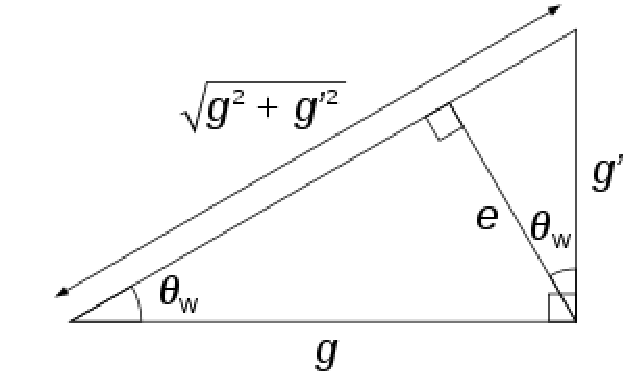
\includegraphics[width=5cm]{Chapter1/Weinberg_angle_relation_between_coupling_constants.pdf}
    \caption{\label{fig:Weinberg_angle} $W^{{\mu}3}$-$B^{\mu}$ plane}
  \end{figure}
\end{minipage}

\noindent obtained by considering a plane in $W_{\mu}^{3}-B_{\mu}$ with $W_{\mu}^{3}$ along x-axis and $B_{\mu}$ along y-axis. The relation among
$\theta_{W}$, $g$ and $g^{\prime}$ is obtained as 
\begin{equation}
  \begin{split}
& \cos{\theta_{W}} = \frac{g}{\sqrt{g^{2} + g^{{\prime}2}}} \hspace{0.2in} ; \hspace{0.2in} \sin{\theta_{W}} = \frac{g^{\prime}}{\sqrt{g^{2} + g^{{\prime}2}}}
  \label{eg:theta_w}
  \end{split}
\end{equation}
Also, using \eqn{\ref{eg:EWK_jmu_all}}, the following relation between $e$, $g$ and $g^{\prime}$ holds,
\begin{equation}
e = g\sin{\theta_{W}} = g^{\prime}\cos{\theta_{W}}
\label{eg:e_g_gprime}
\end{equation}

Thus, the gauge invariance has been restored, but no required mass term appears for the gauge bosons.
Any mass term like $m^{2}W^{\mu}W_{\mu}$ will break the gauge invariance. This hints towards an underlying mechanism,
which provide the masses to gauge bosons alongwith keeping the theory renormalizable and gauge invariant. This mechanism is
known as Higgs mechanism~\cite{Higgs:1964ia, Higgs:1964pj, Higgs:1966ev, Englert:1964et, Guralnik:1964eu}.

\noindent
\underline{\bf{Higgs mechanism:}} The higgs mechanism to endow the gauge bosons with mass has been developed on the idea of
``spontaneous symmetry breaking''~\cite{Djouadi:2005gi} which considers the breaking of a symmetry of a physical system such that
the underlying laws remains invariant under the symmetry transformation, but the physical system itself changes. It is a spontaneous
action that changes the system from a symmetrical state to an asymmetrical state.  

To realize this, a complex scalar field Lagrangian, gauge invariant under $SU(2)$ $\times$ $U(1)$ has been introduced into the electroweak theory
using the same covariant derivative defined in
\eqn{\ref{eg:EWKdelToD}}.
\begin{equation}
\mathcal{L}_{\Phi} = {(D_{\mu}\Phi)}^{\dag}D^{\mu}\Phi - \mu^{2}\Phi^{\dag}\Phi - \lambda{(\Phi^{\dag}\Phi)}^{2}
\label{eq:HiggsLag}
\end{equation}
where $\Phi$ is a $SU(2)$ $\times$ $U(1)$ multiplet of complex scalar fields having weak isospin, $T$ = $1/2$ and weak hypercharge, Y = 1:
\begin{equation}
\Phi = \left(\begin{array}{c} \phi^{+} \\ \phi^{0} \end{array}\right) = \frac{1}{\sqrt{2}} 
 \left(\begin{array}{c} \phi_{1} + i\phi_{2} \\ \phi_{3} + i\phi_{4}  \end{array}\right)
\end{equation}
The potential term of the Lagrangian, $V(\Phi)$ = $\mu^{2}\Phi^{\dag}\Phi + \lambda{(\Phi^{\dag}\Phi)}^{2}$ has two parameters, $\mu^{2}$ and $\lambda$, that
decide its nature. The four particle coupling $\lambda$ specifies the self interactions among the $\phi$ fields and is always positive. We have two
choices for $\mu^{2}$: $\mu^{2}$ $>$ $0$ and $\mu^{2}$ $<$ $0$. For positive $\mu^{2}$, $V(\Phi)$ has a minimum at $\Phi$ = $0$ and the Lagrangian describes
the QED interaction among scalar particles, but for negative $\mu^{2}$,
the potential behaves differently with ground state exhibited by, $\Phi^{\dag}\Phi$ = $\frac{-\mu^{2}}{2\lambda}$ = $\frac{v^{2}}{2}$, in a multi-dimensional regime.
The corresponding potential for real scalar fields before and after symmetry breaking is presented in \fig{\ref{fig:Higgs_potential}}.

Choosing one particular minimum will break the symmetry spontaneously. We choose a ground state where $\phi_{3}$ = $v$, $\phi_{1}$ = $\phi_{2}$ = $\phi_{4}$ = 0 so that
\begin{equation}
\Phi =\frac{1}{\sqrt{2}}\left(\begin{array}{c} 0 \\ v \end{array}\right), \:\:\: \textrm{with } v =\frac{\mu}{\sqrt{\lambda}}
\end{equation}

\begin{figure}[htpb]
\centerline{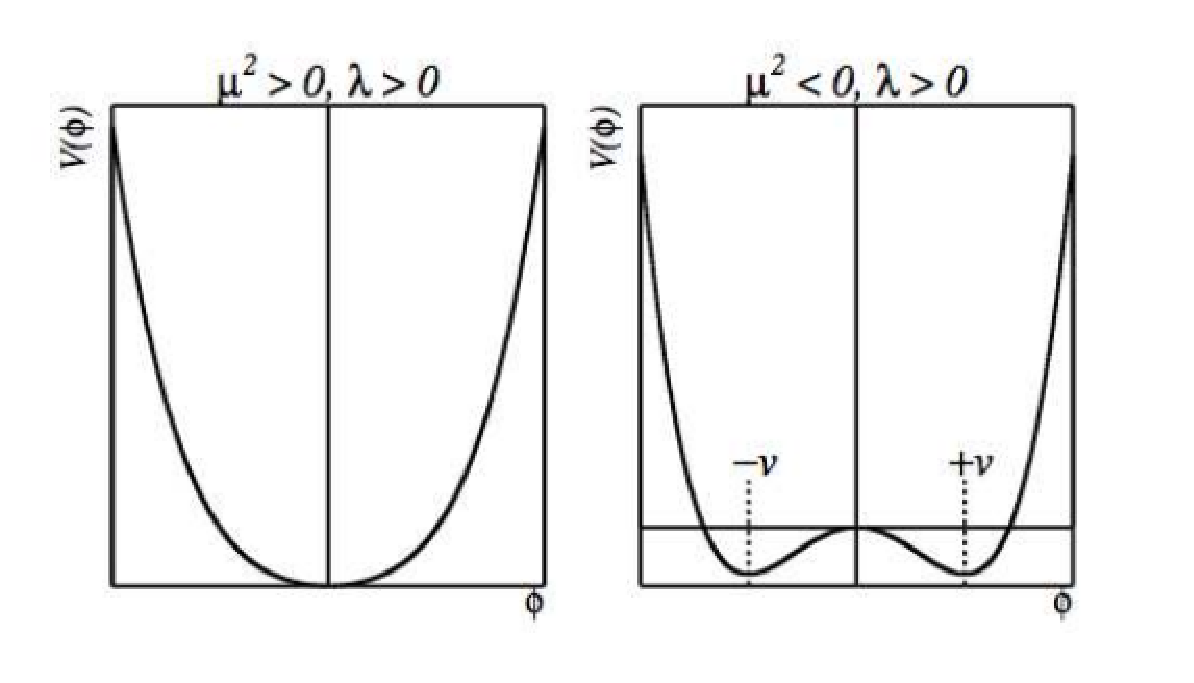
\includegraphics[width=11cm]{Chapter1/Higgs_potential.pdf}}
\caption{A potential with real scalar field $V(\phi)$ = $\mu^{2}\phi^{2}$ + $\lambda{\phi^{4}}$ before and after spontaneous symmetry breaking.}
\label{fig:Higgs_potential}
\end{figure}
\vspace{0.1in}

\noindent This particular choice will break both $SU(2)_{L}$ and $U(1)_{Y}$ gauge symmetries but maintain the $U(1)_{em}$ gauge symmetry. Thus the vacuum state remain invariant
under $U(1)_{em}$ and photon does not acquire any mass. We perturb this field by considering small quantum fluctuations $h(x)$, $h_{1}(x)$, $h_{2}(x)$ and $h_{4}(x)$
corresponding to $\phi_{3}$, $\phi_{1}$, $\phi_{2}$ and $\phi_{4}$ fields respectively, such that
\begin{equation}
  \Phi(x) = \frac{1}{\sqrt{2}} \left(\begin{array}{c} h_{1}(x) + i h_{2}(x) \\ v + h(x) + i h_{4}(x) \end{array}\right)
  \label{eq:Higgs_phi_final}
\end{equation}
Substituting this value of $\Phi$ in the Lagrangian and using the relations defined in \eqns{\ref{eq:EWK_Zmu_Amu},~\ref{eg:theta_w}} and~\ref{eg:e_g_gprime} results into,
\begin{equation}
  \mathcal{L}_{\Phi} = \frac{1}{2}(\partial_{\mu}h)^{2}  + \frac{1}{4}g^{2}(v+h)^{2}(W^{{\mu}+}W_{-}^{\mu}) + \frac{1}{8}(g^{2} + g^{{\prime}2})(v+h)^{2}Z^{\mu}Z_{\mu}
                       - {\lambda}v^{2}h^{2} - {\lambda}vh^{3} - \frac{{\lambda}h^{4}}{4} + \frac{{\lambda}v^{4}}{4}
\end{equation}
This Lagrangian consists of gauge invariant massive higgs field $h$ with mass, $m_{h}$ = $\sqrt{2{\lambda}v^{2}}$, along with the mass terms
for weak gauge bosons $W_{\mu}^{\pm}$ and $Z_{\mu}$. It can be seen that there is no mass term for photon field $A_{\mu}$.
\begin{equation}
  M_{W^{\pm}} = \frac{1}{2}gv, \hspace{0.2in} M_{Z} = \frac{1}{2}v{\sqrt{g^{2} + g^{{\prime}2}}}; \hspace{0.2in} M_{A} = 0 
\end{equation}
Thus, the spontaneous breaking of gauge symmetry has resulted into the generation of masses of weak gauge bosons. The other terms of the Lagrangian represents
the interaction terms of the higgs field with gauge bosons. The same higgs field also provide the masses to fermions through Yukawa coupling defined by,
\clearpage
\begin{equation}
  \mathcal{L}_{Yukawa} = -y_{l}\bar{L}{\phi}e_{R} -y_{u}\bar{Q}(-i{\sigma}_{2}){\phi}^{\ast}u_{R} -y_{d}\bar{Q}{\phi}d_{R} + h.c.
  \label{eq:Yukawa_coup}
\end{equation}
with $y_{l,u,d}$ being Yukawa coupling constants and ${u}_{R}$, ${d}_{R}$ (${e}_{R}$) being the left-handed doublet and right-handed singlet quark (lepton) fields.
Now again we break the symmetry and perturb the system around the minima to obtain a value for field $\Phi$ defined in \eqn{\ref{eq:Higgs_phi_final}}. Using it in the
Lagrangian gives,
\begin{equation}
  \mathcal{L}_{Yukawa} = -\frac{1}{\sqrt{2}}y_{l}\bar{l}_{L}(v+h)l_{R} -\frac{1}{\sqrt{2}}y_{q}\bar{q}_{L}(v+h)q_{R},
\end{equation}
where $l_{L,R}$ and $q_{L,R}$ denote the lepton and quark fields. We see that a mass term for fermions appears in this lagrangian given by, $m_{f}$ = $\frac{1}{\sqrt{2}}y_{f}v$, showing that the coupling strength $y_{f}$ of fermions with higgs field is
proportional to the mass of fermion. 

Thus, the full electroweak Lagrangian is a sum of four terms,
\begin{equation}
  \mathcal{L}_{EWK} = \mathcal{L}_{fermion} + \mathcal{L}_{K.E.} + \mathcal{L}_{\Phi} + \mathcal{L}_{Yukawa}
\end{equation}
 
\subsubsection{Quantum chromodynamics}
The theory of strong force, known as Quantum chromodynamics, has also been developed on the steps of QED. Since quarks come in three colors, in contrast to the single
charge of QED photon, the gauge group considered is SU(3), an extension of $U(1)$ gauge group in 3-dimension. It is a non-abelian gauge theory
with quark's color fields forming the fundamental representation. The Lagrangian for free quark fields can be written as,
\begin{equation}
\mathcal{L}_{q} = \sum_{j = 1,2,3} \overline{q}_{j}(x)(i\gamma^{\mu}\partial_{\mu} - m){q_{j}}(x)
\label{eq:QCDLang}
\end{equation}
This Lagrangian is conserved under the global phase transformation with the conserved currents, $j_{\mu}^{c}$ = $\sum_{j = 1,2,3} g\overline{q}_{j}\gamma^{\mu}T_{a}q_{j}$,
known as color charge densities. Considering the invariance of Lagrangian under the local gauge transformations,
\begin{equation}
q_{j}(x) \rightarrow q_{j}^{\prime}(x) = e^{i{\alpha}_{a}(x)T_{a}}q_{j}(x) 
\label{eg:QCDLocalphase}
\end{equation}
where $T_{a}$, $a$ = $1,2,\ldots,8$ are the generators of $SU(3)$ transformations with $[T_{a}, T_{b}]$ = $if_{abc}T_{c}$, $f_{abc}$ are anti-symmetric
real structure constants. To make Lagrangian invariant under this local phase, we introduce the 
following covariant derivatives and fields,
\begin{equation}
  D_{\mu} = \partial_{\mu} + igT_{a}G_{\mu}^{a} \hspace{0.2 in} ; \hspace{0.4 in} G_{\mu}^{a} \rightarrow G_{\mu}^{a} - \frac{1}{g}\partial_{\mu}\alpha_{a}(x) -
  f_{abc}\alpha_{b}(x)G_{\mu}^{c} 
\label{eg:QCDdelToD}
\end{equation}
where last term of $G_{\mu}^{a}$ signifies the non-abelian nature of the theory. Substituting $\partial_{\mu}$ $\rightarrow$ $D_{\mu}$ in the Lagrangian,
\begin{equation}
\mathcal{L}_{q} \rightarrow \mathcal{L}'_{q} = \mathcal{L}_{q} - \sum_{j = 1,2,3} g\overline{q}_{j}\gamma^{\mu}T_{a}G_{\mu}^{a}{q_{j}} 
  \label{eq:QCDLang_Dmu}
\end{equation}
Also, considering the kinetic energy term for the gauge fields, $G_{\mu}^{a}$, we can write the complete QCD Lagrangian as,
\begin{equation}
  \mathcal{L}_{q} = \sum_{j = 1,2,3} \overline{q}_{j}(x)(i\gamma^{\mu}\partial_{\mu} - m){q_{j}}(x) - g\overline{q}_{j}\gamma^{\mu}T_{a}G_{\mu}^{a}{q_{j}} -
  \frac{1}{4}G_{\mu\nu}^{a}G^{{\mu\nu}a}
  \label{eq:QCDLang_final}
\end{equation}
where,
\begin{equation}
  G_{\mu\nu}^{a} = \partial_{\mu}G_{\nu}^{a} - \partial_{\nu}G_{\mu}^{a} - gf_{abc}G_{\mu}^{b}G_{\nu}^{c}
  \label{eq:Gmunu_QCD}
\end{equation}

Thus, we can see that the invariance of Lagrangian under local gauge has resulted into the appearance of interaction fields into the theory with the mediators
of interaction, gluons, remaining massless.

%%%%%%%%%%%%%%%%%%%%%%%%%%%%%%%%%%%%%%%%%%%%%%%%%%%%%%%%%%%%%%%%%%%%%%%%%%%%%%%%%%%%%%%%%%%%%%%%%%%%%%%%%%%%%%%%%%%%%%%%%%%%%%%%%%%%%%%%%%%%%%%%%%%%%%%%%%%%%%%%%%%%%%%%%%
%% \subsubsection{Grand unification theory}                                                                                                                             %%
%% The standard model predicts the existence of a unified theory of electroweak and strong interactions, known as Grand Unified Theory (GUT).                           %%
%% The grand unification is believed to have existed at very high energies at the beginning of the universe. This theory unifies the three fundamental forces into one  %%
%% under a grand unified gauge group $\mathcal{G}$,                                                                                                                     %%
%% \begin{equation}                                                                                                                                                     %%
%%   SU (3)_{C} \times SU (2)_{L} \times U (1)_{Y} \subset \mathcal{G}                                                                                                  %%
%%   \label{eq:GUT}                                                                                                                                                     %%
%% \end{equation}                                                                                                                                                       %%
%% where the gauge transformations in $\mathcal{G}$ relate the couplings $g$ and $g^{\prime}$ of electroweak interaction to the strong coupling $\alpha_{s}$.           %%
%% All the three interactions are then interpreted by a single gauge group $\mathcal{G}$ and single coupling $g_{\mathcal{G}}$,                                         %%
%% with $g_{\mathcal{G}}$ relating to $g$, $g^{\prime}$ and $\alpha_{s}$ in some specific ways.                                                                         %%
%% However, an exact form of the grand unification group $\mathcal{G}$ and corresponding symmetries are yet to be found out.                                            %%
%% One of the predictions of the GUTs is the decay of protons. Since no proton decays has been observed yet, it ruled out the existence of simple GUTs, like $SU(5)$ or %%
%% $SO(10)$.                                                                                                                                                            %%
%%                                                                                                                                                                      %%
%% Also, there is no quantized theory of gravitation yet, still a Theory of Everything (TOE) unites the theory of quantum gravity and GUT as well                       %%
%% into one common framework.                                                                                                                                           %%
%%%%%%%%%%%%%%%%%%%%%%%%%%%%%%%%%%%%%%%%%%%%%%%%%%%%%%%%%%%%%%%%%%%%%%%%%%%%%%%%%%%%%%%%%%%%%%%%%%%%%%%%%%%%%%%%%%%%%%%%%%%%%%%%%%%%%%%%%%%%%%%%%%%%%%%%%%%%%%%%%%%%%%%%%%

\subsection{Challenges faced by SM:\ unknown mysteries}
The standard model is acknowledged to be the most successful theoretical model till today. Over the years, it has been built up owing to the lively
conversations between theoretical predictions and experimental proofs. Even after being able to describe so many natural phenomena, this model is not
considered perfect. The reason being several existing questions that standard model can not adequately explain. Some of these include:
\vspace{-0.15in}
\begin{itemize}
   \setlength\itemsep{0.03em}
\item {\bf{Gravity}}: Standard model does not include gravity and provides no explanation for it.
\item {\bf{Three generations}}: No particular justification has been given in SM as to why only three particle generations exist and why there is so much variation
  in masses of particles from different generations.
\item {\bf{Neutrino mass}}: In SM, neutrinos are regarded as massless. However, there are many experimental
  results~\cite{Fukuda:2001nk, Fukuda:1998mi, Araki:2004mb, Aliu:2004sq} which prove that neutrinos have small tiny non-zero mass.
\item {\bf{Matter-Antimatter asymmetry}}: The imbalance of matter and anti-matter within the observable universe, also referred to as baryon asymmetry,
  has been one of the greatest mysteries of particle physics for which standard model has no answer.
\item {\bf{Dark energy and dark matter}}: It has been observed in various cosmological observations that the visible matter accounts for only 5$\%$ of the total
  energy-mass content of the universe. The SM gives no explanation for the rest of about 25$\%$ of the non-luminous dark matter and about 70$\%$ of dark energy.   
\item {\bf{Short range of strong force}}: Usually, the range of a force is inversely proportional to the mass of its mediator. But this is not true for
  strong force. Its mediators, gluons are massless, still, this force is of limited range. No explanation for this is provided in SM. 
\end{itemize}
\vspace{-0.2in}
So the picture depicted by SM is not perfect, it has been, therefore, regarded as a piece of a bigger picture that will be explained by
some beyond the standard model theories. 

\section{Beyond The Standard Model}
Many theoretical models have been developed to overcome the deficiencies observed in standard model. These models are collectively known as ``Beyond the Standard Model''
(BSM) theories. The most famous among these are String theory, Supersymmetry, Technicolor, compositeness etc.
\subsection{Model of excited quarks}
The study represented in this thesis is based on a model that considers the excited state of quarks ($\qstar$) and leptons ($\lstar$),
also known as compositeness models~\cite{Pati:1975md, Eichten:1983hw, Baur:1987ga, Baur:1989kv}.
The prime motivation for these models are the presence of three quark and lepton generations with similar properties. This replication points toward
some underlying structure identical in all the families. The most implicit signature of this sub-structure is the observation of a fermion (quark or lepton)
in the excited state. The analogy with excited states has been made on the basis of a very basic physics phenomena. We know that a composite system,
e.g.\ a hydrogen atom, consists of various energy levels arising due to the interactions among its constituents. Thus, the
observation of a system in excited state is the confirmation of its composite structure.
The excited state of fermions is assumed as a resonance state which then eventually decay into SM particles. 

The fundamental particles that quarks and leptons are considered to be composed of, are known as ``preons''. These preons are postulated to experience a new kind of
force that becomes very strong at a particular scale $\Lambda$, known as the compositeness scale, forming quarks and leptons bound states. 
Excited quarks and leptons can interact with their ordinary counterparts through contact interactions for $\Lambda$ $>>$ $\sqrt{\shat}$ and through gauge
mediation for $\Lambda$ $<$ $\sqrt{\shat}$ where $\sqrt{\shat}$ is the center of mass energy. The model used in this study assumes compositeness scale $\Lambda$
$<$ $\sqrt{\shat}$ and mass scale of excited quarks $M_{\qstar}$ = $\Lambda$, gauge interactions dominate over contact interactions in this regime.
The excited quark model used in this study~\cite{Baur:1989kv} considers a $SU(3)$ $\times$ $SU(2)$ $\times$ $U(1)$ symmetry with ground state quarks in the
form of left-handed doublets and right-handed singlets while the excited quarks in the form of left- and right-handed doublets. 
\begin{equation}
\textrm{Ground state: }\left(\begin{array}{c} u \\ d \\ \end{array} \right)_{L}
\hspace{0.1cm}, \hspace{0.1cm} u_{R}, \hspace{0.1cm} d_{R} \hspace{0.5in}
\textrm{Excited state: }\left(\begin{array}{c} \ustar \\ \dstar \\ \end{array} \right)_{L}
\hspace{0.1cm}, \hspace{0.1cm} \left(\begin{array}{c} \ustar \\ \dstar \\ \end{array} \right)_{R}
\end{equation}
The excited quarks interact with gauge bosons via vectorlike coupling defined by the Lagrangian:
\begin{equation}
\mathcal{L}_{gauge} = \bar{q^{\star}}\gamma^{\mu} \left[ g_{s}\frac{\lambda^{a}}{2}G_{\mu}^{a} + g\frac{\tau^{b}}{2}W_{\mu}^{b} + g'\frac{Y}{2}B_{\mu} \right]q^{\star}
\end{equation}
where $g_{s}$, $g$, and $g^{\prime}$ are the coupling constants for strong and electroweak interactions; $G_{\mu}^{a}$, $W_{\mu}$, and $B_{\mu}$ denote
the gauge fields corresponding to $SU(3)$, $SU(2)$, and $U(1)$ gauge groups. The excited quarks attain spin and isospin value of $\frac{1}{2}$ and weak hypercharge
$Y$ value of $\frac{1}{3}$ under this model. The gauge interaction mediated between ordinary and excited quarks by gauge bosons is obtained through the
requirement of gauge invariance and is of magnetic-moment type, defined by the effective Lagrangian:
\begin{equation}
{\mathcal L}_{int} = \frac{1}{2\,\Lambda}\bar{q^{\ast}_{R}} \, \sigma^{\mu\nu}
\left[g_{s}f_{s}\frac{\lambda^{a}}{2}G^{a}_{\mu\nu}\;+\;gf\frac{\tau^{b}}{2}W_{\mu\nu}^{b}\;+\;g'f'\frac{Y}{2}B_{\mu\nu} \right] q_{L} + h.c.,
\label{eq:Lagrangian1}
\end{equation}
Here $G^{a}_{\mu\nu}$, $W_{\mu\nu}$, and $B_{\mu\nu}$ are corresponding field-strength tensors while $\lambda_{a}$, $\tau_{b}$, $Y$
are the corresponding generators for $SU(3)$, $SU(2)$, and $U(1)$ fields. The constants $f_{s}$, $f$, $f'$ determine the strength of a coupling and are
evaluated using the compositeness dynamics, these are considered to be equal to unity to allow for the standard model like coupling strengths. 

A composite quark can acquire an excited state by the absorption of a gluon and will radiate a photon, gluon or weak boson on returning to the ground state.
The branching fractions of excited quark decays into various final states is given in the \tab{\ref{Table:qstarBR}} below.
%---------------TABLE FOR MC samples-------------------
\begin{table}[h!]
\begin{center}
%\begin{ruledtabular} 
  %\resizebox{7cm}{!}{
\renewcommand{\arraystretch}{1.2}
\begin{tabular}{lr}
\toprule
\belowrulesepcolor{Mygray}
\belowrulesepcolor{Mygray}
\belowrulesepcolor{Mygray}
\rowcolor{Mygray}[\dimexpr\tabcolsep+0.09pt\relax]
Decay Channel \hspace{0.5in}      & BR     \\
\aboverulesepcolor{Mygray}
\aboverulesepcolor{Mygray}
\aboverulesepcolor{Mygray}
\midrule
$\qstar\to$qg       \hspace{0.5in} & $\sim$ 83\% \\
$\qstar\to$q$\gamma$\hspace{0.5in} & $\sim$ 2\%  \\
$\qstar\to$q$Z^{0}$ \hspace{0.5in} & $\sim$ 5\%  \\
$\qstar\to$q$W^{-}$ \hspace{0.5in} & $\sim$ 10\%  \\
\bottomrule
\end{tabular}
%}
\caption{Approximate estimate of branching fractions (BR) of \qstar\ decay in different channels, assumptions made are: $\Lambda$ = $M_{\qstar}$ and $f$ = $f^{\prime}$ = $f_{s}$.}
%\end{ruledtabular}
\label{Table:qstarBR}
\end{center}
\end{table}
%\vspace{-0.3in}

\vspace{-0.3in}

This study considers an excited light ($\ustar,\dstar$) and heavy ($\bstar$) flavor quark decaying into a quark and a photon final state.
The physics processes contributing to this final state are represented in the form of Feynman diagrams in the \fig{\ref{fig:qstarSig}}
with $q$ referring to $u, d$ and $b$ quark.
%\vspace{-0.2in}
\begin{figure}[h]
\begin{center}
\subfloat[qg fusion]{\label{fig:qgFusion}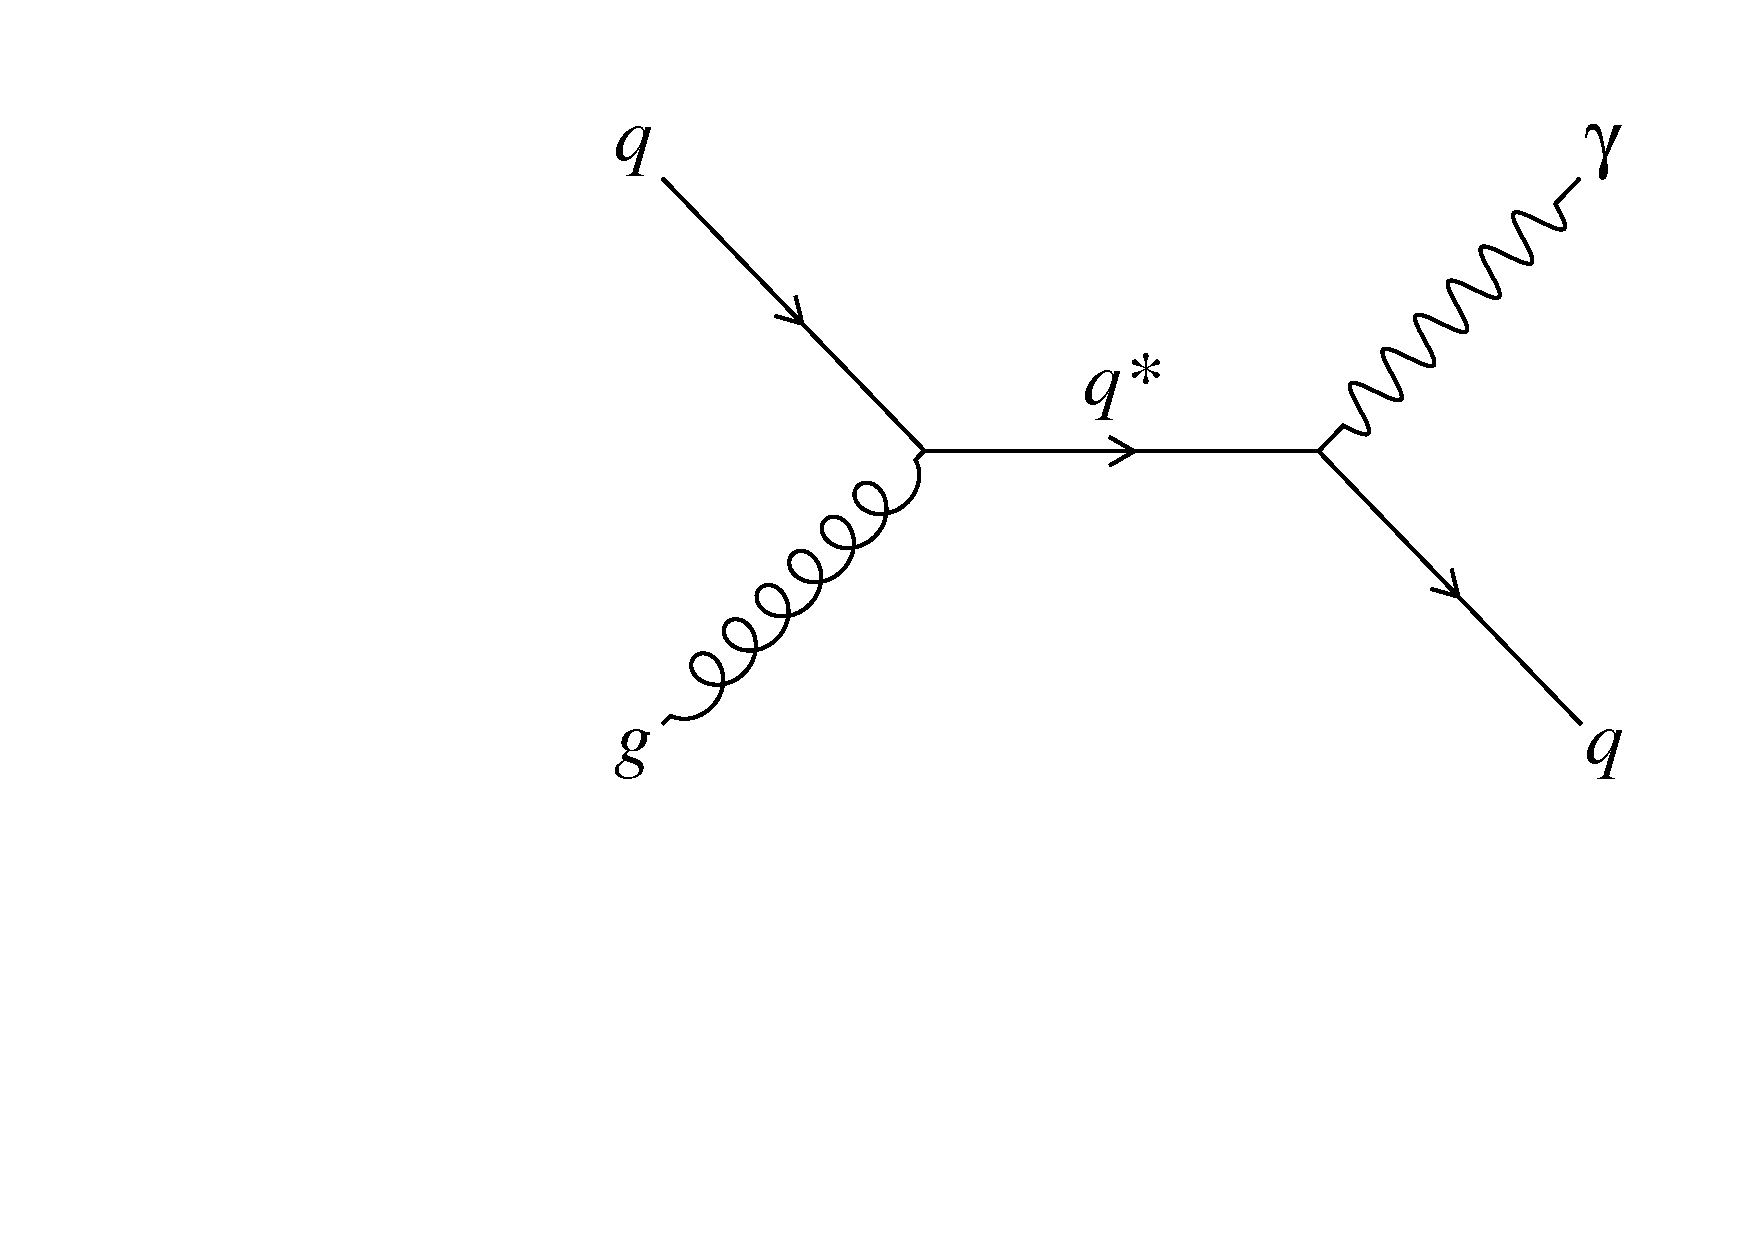
\includegraphics[width=4.6cm]{Chapter1/Feynman_diagrams/Signal_qgFusion.pdf}}
\hspace{0.1 in}
\subfloat[q$\bar{\textrm{q}}$ annihilation]{\label{fig:qqbarAnni}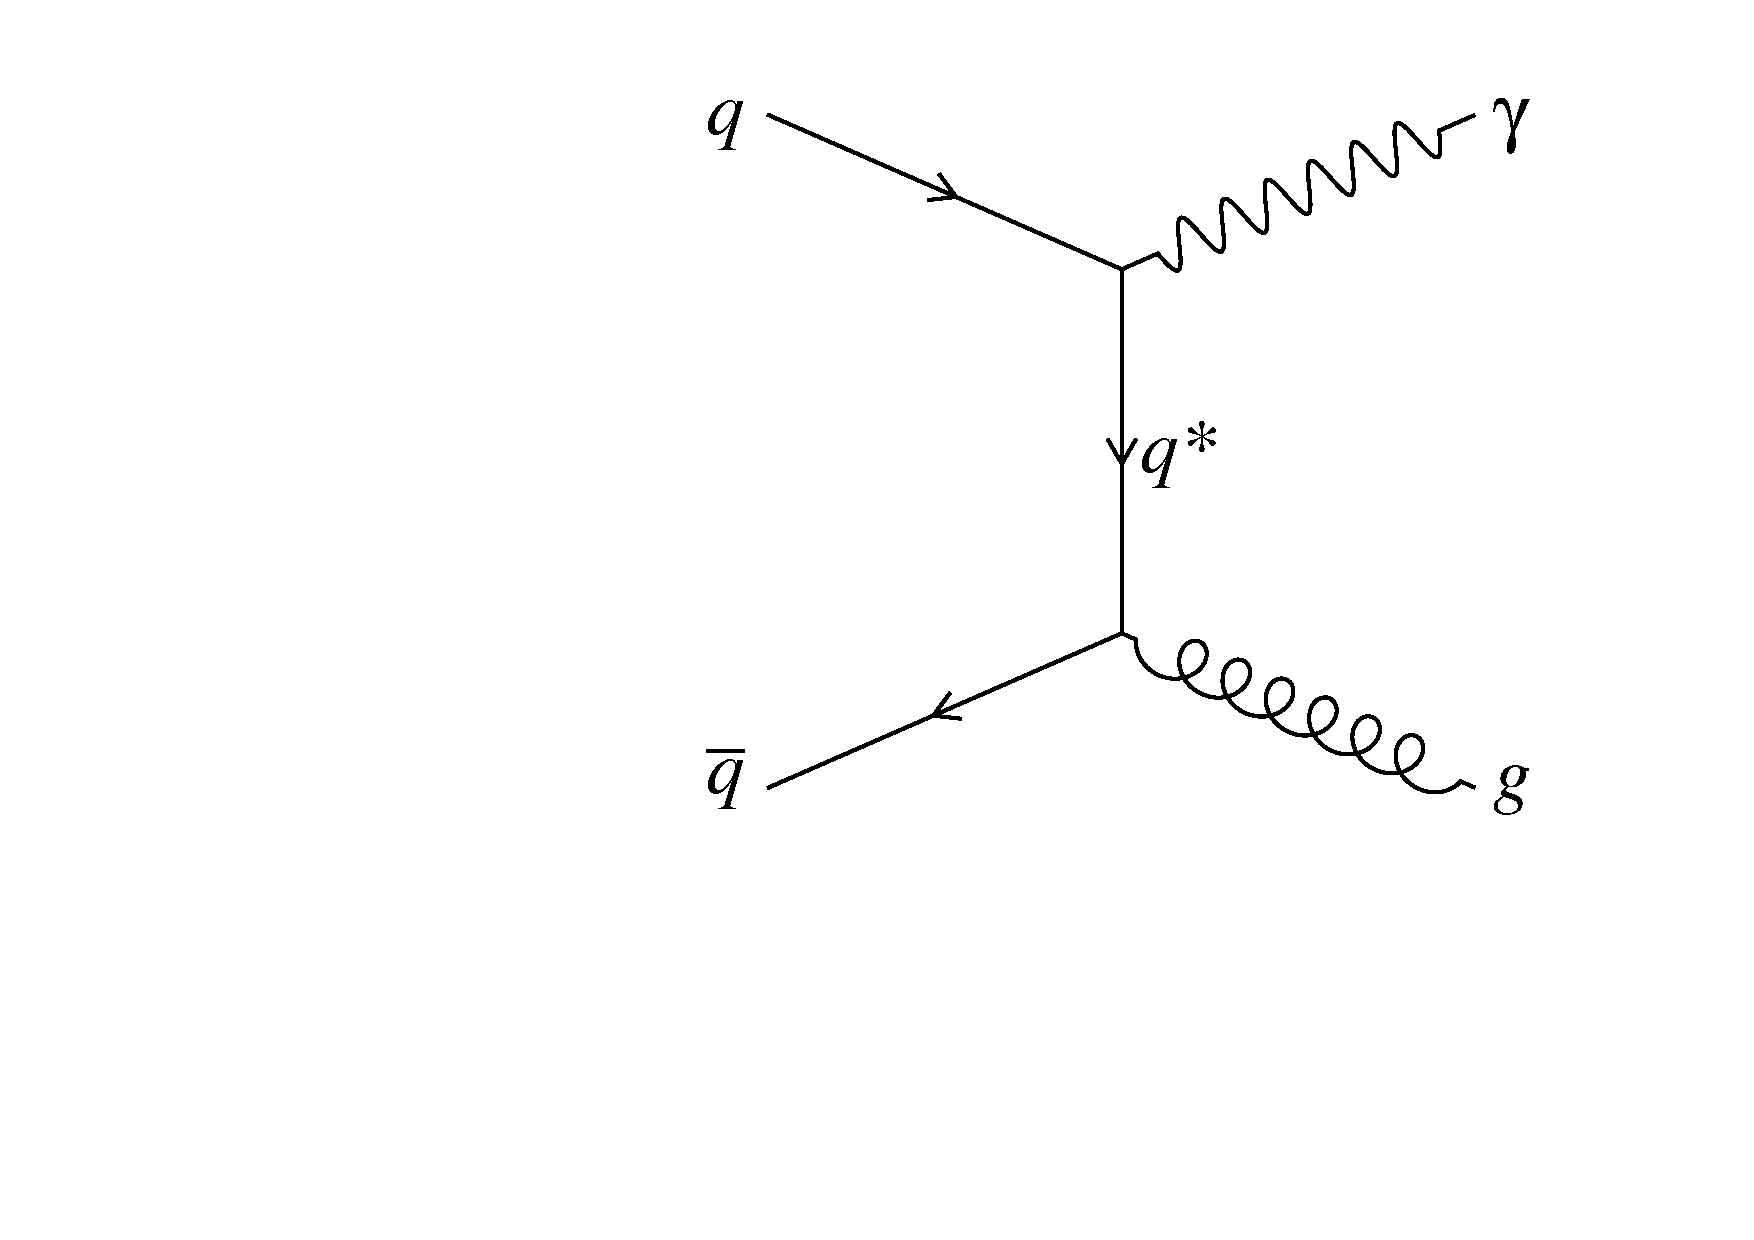
\includegraphics[width=4.4cm]{Chapter1/Feynman_diagrams/Signal_qqbarAnnihilation.pdf}}
\hspace{0.1 in}
\subfloat[gg fusion]{\label{fig:ggFusion}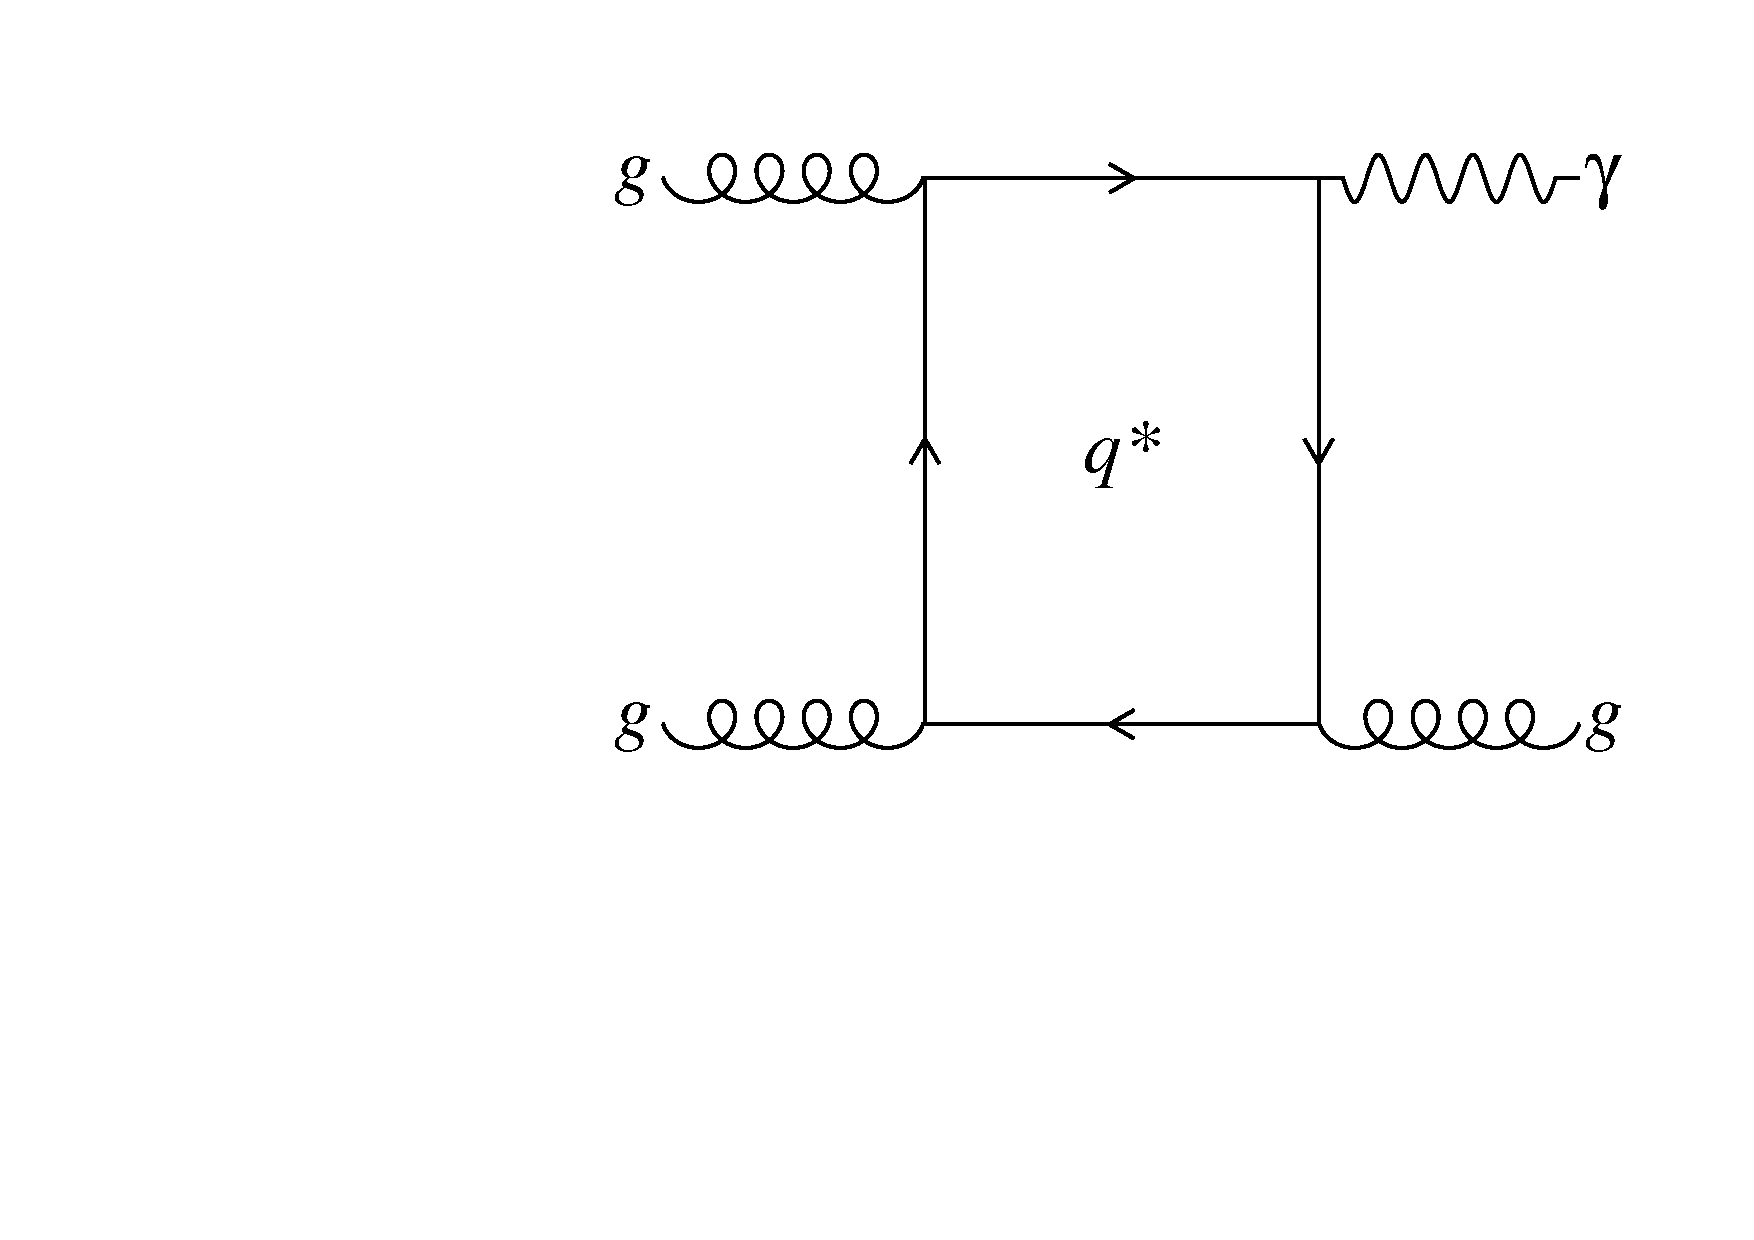
\includegraphics[width=4.4cm]{Chapter1/Feynman_diagrams/Signal_ggFusion.pdf}}
\caption{Feynman diagrams for $\qstar$ $\rightarrow$ $\gamma$ + jet final state with (a) quark-gluon fusion (b) quark-antiquark annihilation
  (c) gluon-gluon fusion processes. Whereas the light quarks will show their presence in all the three modes, heavy bottom quark will appear only in quark-gluon fusion and quark-antiquark annihilation.}
\label{fig:qstarSig}
\end{center}
\end{figure}
\vspace{-0.3in}

Under the assumption $\Lambda$ $<$ $\sqrt{\shat}$, gauge interactions will be dominating and the excited quarks will be produced mainly via the
s-channel\footnote{s,t and u are called Mandelstam variables. For a $2-2$ scattering process
  of initial momenta p$_{1}$ and p$_{2}$ and final momenta p$_{3}$ and p$_{4}$, the variables are defined as, s = (p$_{1}$ + p$_{2}$)$^{2}$ = (p$_{3}$ + p$_{4}$)$^{2}$,
  t = (p$_{1}$ $-$ p$_{3}$)$^{2}$ = (p$_{4}$ $-$ p$_{2}$)$^{2}$ and u = (p$_{1}$ $-$ p$_{4}$)$^{2}$ = (p$_{3}$ $-$ p$_{2}$)$^{2}$. Each one represents a different
  Feynman diagram of a process.}
quark-gluon fusion process. The scattering of an ordinary quark and gluon in s-channel
will produce an excited quark resonance that will tower over the continuous SM $\gamjet$ background. Appearance of excited quark in other channels will be
captured in the form of excess of events over the background distribution. 

\subsection{A follow-up of previous searches}
Many attempts have been made in the past to look for the evidences of quark compositeness. But no success has been gained yet.
A summary of the various experiments that deployed their potential in this important search are reported here. 

The ZEUS detector at HERA looked for excited quarks of heavy flavor in $e^{+}p$ collisions at $\sqrt{s}$ = 300\unit{GeV} and excluded the excited quarks
in the mass range 40-169\unit{GeV} at the 95$\%$ confidence level (CL)~\cite{Breitweg:1997qa}. 

The CDF detector collaboration at Tevatron also searched for excited quarks in \gamjet\ and
dijet channels in $\textrm{p}\bar{\textrm{p}}$ collisions at center of mass
energy of 1.8 TeV and excluded the ranges $80<\mqstar<540\unit{GeV}$~\cite{CDFexclgj}, $200<\mqstar<520\unit{GeV}$ \nd\
$580<\mqstar<760\unit{GeV}$~\cite{CDFexcljj}, respectively. The D0 collaboration at Tevatron looked for evidence in dijet final state~\cite{D0excl}
and excluded $M_{\qstar}$ below 775\unit{GeV} at 95\% CL.\ The CMS and ATLAS Collaborations have also performed the searches in $\textrm{pp}$ collisions
at $\sqrt{s}$ = 7\unit{TeV}, 8 \unit{TeV} as well as 13\unit{TeV}. At $\sqrt{s}$ = 8\unit{TeV}, exclusions have been reported by both the collaborations
in different channels. At $\sqrt{s}$ = 13\unit{TeV}, ATLAS had excluded $\qstar$ below 5.2\unit{TeV}
with 95$\%$ CL in the dijet channel~\cite{ATLAS:2015nsi} and below 4.4\unit{TeV} in the $\gamjet$ channel~\cite{Aad:2015ywd}. The CMS Collaboration
has also excluded excited quarks below 5.0\unit{TeV} in the dijet channel~\cite{Khachatryan:2015dcf}.

Searches for excited states of heavy bottom quarks have also been performed earlier in different channels.
The ATLAS collaboration searched for $\bstar$ in $tW$ final state at $\sqrt{s}$ = 7\unit{TeV}~\cite{Aad:2013rna} and excluded $M_{\bstar}$ for masses below 870\unit{GeV}.
The CMS collaboration have looked for excited b-quarks in $tW$ and dijet final state at $\sqrt{s}$ = 8\unit{TeV}. In $tW$ final state, it excluded
$\bstar$ upto the masses of 1.53\unit{TeV} for vector-like couplings~\cite{Khachatryan:2015mta} at 95$\%$ CL while in
dijet final state, it claimed an exclusion in the range of
1.20-1.56\unit{TeV}~\cite{Khachatryan:2015sja}. At $\sqrt{s}$ = 13\unit{TeV}, no search for $\bstar$ has been performed yet, this study, therefore, presents the
first search for $\bstar$ at $\sqrt{s}$ = 13\unit{TeV}. 


%\section{Thesis Organization}



%keywords that can be used at any place: turbulence, intellectual, retrospect (a survey of past few years), thence (as a consequence),
  

